\documentclass[a4paper,twoside]{tufte-book}\usepackage[]{graphicx}\usepackage[]{color}
%% maxwidth is the original width if it is less than linewidth
%% otherwise use linewidth (to make sure the graphics do not exceed the margin)
\makeatletter
\def\maxwidth{ %
	\ifdim\Gin@nat@width>\linewidth
	\linewidth
	\else
	\Gin@nat@width
	\fi
}
\makeatother

\usepackage{Sweavel}

%style file is in the same folder.

%\usepackage{ngerman}
\usepackage[T1]{fontenc}
\usepackage[utf8]{inputenc}


\usepackage{color}
\usepackage{xcolor}
\usepackage{framed}
\usepackage{listings}

\usepackage{graphicx}

\usepackage{multicol}              
\usepackage{multirow}
\usepackage{booktabs}
%\usepackage{natbib} 

\usepackage[innerrightmargin = 0.7cm, innerleftmargin = 0.3cm]{mdframed}
\usepackage{mdwlist}

\usepackage[]{hyperref}
\definecolor{darkblue}{rgb}{0,0,.5}
\hypersetup{colorlinks=true, breaklinks=true, linkcolor=darkblue, menucolor=darkblue, urlcolor=blue, citecolor=darkblue}

\usepackage[toc,page]{appendix}


\setcounter{secnumdepth}{1}
\setcounter{tocdepth}{1}

\lstset{ % settings for listings needs to be be changed to R sytanx 
	language=R,
	breaklines = true,
	columns=fullflexible,
	breakautoindent = false,
	%basicstyle=\listingsfont, 
	basicstyle=\ttfamily \scriptsize,
	keywordstyle=\color{black},                          
	identifierstyle=\color{black},
	commentstyle=\color{gray},
	xleftmargin=3.4pt,
	xrightmargin=3.4pt,
	numbers=none,
	literate={*}{{\char42}}1
	{-}{{\char45}}1
	{\ }{{\copyablespace}}1
}
% http://www.monperrus.net/martin/copy-pastable-listings-in-pdf-from-latex
\usepackage[space=true]{accsupp}
% requires the latest version of package accsupp
\newcommand{\copyablespace}{
	\BeginAccSupp{method=hex,unicode,ActualText=00A0}
	\ %
	\EndAccSupp{}
}









\title{Essentielle\\Statistik}
\author{Florian Hartig}


\begin{document}
	%\SweaveOpts{concordance=TRUE} % don't activate this for knitr
	
	\let\cleardoublepage\clearpage % No empty pages between chapters
	\maketitle
	
	
	\thispagestyle{empty}
	\null
	
	\begin{fullwidth}
		Diese Vorlesung ist empfehlenswert für Studenten der
		
		\begin{itemize*}
			\item BSc Biostatistik
			\item MSc Research Skills (Internetpräsenz \href{http://florianhartig.github.io/ResearchSkills/}{siehe hier})
		\end{itemize*}
		
		\vspace{0.5cm}
		
		Anmerkungen / Fragen an:\\[0.5cm]
		\href{https://florianhartig.wordpress.com/}{Florian Hartig}\\
		Universität Regensburg\\
		Germany\\[0.5cm]
		
		Probleme oder Unklarheiten bei dieser Vorlesung können mittels \href{https://github.com/florianhartig/Statistics/issues}{issue tracker} der \href{https://github.com/florianhartig/Statistics/tree/master/EssentialStatistics}{GitHub repository} gemeldet werden. 
		
	\end{fullwidth}
	
	
	\vfill
	\begin{fullwidth}
		Erstellt 2014. Updated 2015. Diese Arbeit fällt unter die 'Creative Commons Attribution-NonCommercial-NoDerivatives 4.0 International' Lizenz.
	\end{fullwidth}
	
	\newpage
	\renewcommand{\contentsname}{Inhalt}
	\tableofcontents
	
	\newpage
	
	\chapter{Einleitung} % Use chapters instead of sections
	
	\section{Absichten und vorgesehene Zielgruppe}
	
	Dieses Dokument beinhaltet eine kurze Einführung in die Statistik und in statistische Analysen, welche in elementaren Experimenten und beobachteten Situationen häufig von Nöten sind~\ref{sec: further readings}.
	
	\section{Themen der Statistik und Datenwissenschaften}
	Statistik, oder auch Datenwissenschaften, behandelt die Visualisierung, Zusammenfassung und Interpretation von Daten. Dieses Skript beinhaltet eine Hinführung an die vier wichtigsten Säulen der statistischen Methodik für einen quantitativen Wissenschaftler:
	
	\paragraph{Deskriptive Statistik:} Deskriptive Statistik\marginnote{Deskriptive Statistik = Plots, Maßzahlen der Statistik} beinhaltet die Maßzahlen der Statistik, wie beispielsweise der Mittel- oder Medianwert, aber auch weitere Optionen, um Daten zu visualisieren.
	
	\paragraph{Inferenzstatistik:} Inferenzstatistik\marginnote{Inferenzstatistik = Parameterschätzungen, p-Werte, Tests} behandelt das Testen von Hypothesen und Schätzen von Parametern. Inferenz basiert typischerweise auf Annahmen, welche in einem statistischen Modell zusammengefasst sind.\marginnote{Ein statistisches Modell beschreibt, wie Daten erstellt werden = Datenerzeugender Prozess} Ein statistisches Modell wird auch als "`Datenerzeugender Prozess"' bezeichnet, da es Annahmen über einen Prozess beschreibt, die zu einer Variation an Daten führt (systematisch und stochastisch).
	
	\paragraph{Vorhersagende Statistik und maschinelles Lernen:} Vorhersagende Statistik und maschinelles Lernen\marginnote{Maschinelles Lernen = Vorhersagende Modelle. Große Dateien = umfangreiche Datensätze, z.\,B. von Amazon-Endkunden} arbeiten mit herleitenden Vorhersagen aus v.\,A. sehr "`großen Dateien"'. Der Hauptunterschied zur Inferenzstatistik ist, dass der Fokus auf der entstehenden Methode liegt, um gute Vorhersagen treffen zu können ohne ein vorhergehendes Beschreiben, Folgern oder Testen von Annahmen über den Datenerzeugenden Prozess.
	
	\paragraph{Experimentelle Planung:} Experimentelle Planung\marginnote{Experimentelle Planung oder Analysenplanung = das Erhalten und Erzeugen von Daten} umfasst alle Aspekte der Datenerzeugung, insbesondere Fragen wie "`Welche Variablen sollten erfasst werden?"', "`Wie viele Replikate werden benötigt?"', "`Wie sollten die Variablen in einem Experiment optimalerweise verändert werden?"'
	
	
	\section{Die Umgebung R für statistische Berechnungen}
	
	Die Zeiten als Statistik noch mit Stift, Papier und Taschenrechner durchgeführt wurde sind nun mehr oder weniger vorbei. Heutzutage werden statistische Analysen am Computer durchgeführt, wofür es eine Reihe von Software-Umgebungen gibt.
	
	In diesem Skript werden alle Beispiele mit Hilfe von R berechnet werden; wobei der Fokus jedoch nicht auf einer Einführung in R an sich liegen wird. Bei Bedarf führt  \href{http://biometry.github.io/APES/R/R10-gettingStarted.html}{dieser Link} zu einer Einführung, inklusive Hilfestellungen für die Installation der Software.
	
	\begin{figure}[]
		\begin{center}
			\includegraphics[width = 10cm]{rst_interface.png}
			\caption{Der RStudio Editor ist der wohl beliebteste Editor für R. R ist eine script-basierende Sprache. Hier kommuniziert man nicht durch Klicken mit dem Computer, sondern gibt Anweisungen anhand von direkten Befehlen in die R Konsole, oder durch das vorhergehende Anlegen eines Text-Dokuments, welches dann die Befehle auswertet. Wenn man diese Herangehensweise nicht gewöhnt ist, kann es eine Weile dauern, bis man damit warm wird. Wenn man sich jedoch damit angefreundet hat, wird man bald merken, wie komfortabel und vorteilhaft es ist, alle Schritte der Analyse in einem Textdokument aufgelistet wiederzufinden und somit alles zu jeder Zeit nachvollziehen zu können.}
			\label{fig: Rstudio}
		\end{center}
	\end{figure}
	
	
	
	\chapter{Dateien, Proben und Populationen}
	
	Die folgenden vier Kapitel sind den vier Typen der statistischen Analyse zugewiesen, die in der Einleitung bereits genannt wurden: deskriptive Statistik, Inferenzstatistik, vohersagende Statistik und experimentelle Planung. 
	
	\section{Stichproben, Populationen und der Vorgang der Datenerzeugung}
	
	Der eigentliche Grund der für statistische Berechnungen spricht, ist, dass die Daten, die wir erhalten, sehr zufällig erscheinen. Aber wie entsteht diese Zufälligkeit?
	
	Man stelle sich vor, \marginnote{Eine Population ist die Zusammenstellung aller Beobachtungen, die man hätte machen können. Eine Stichprobe ist die Beobachtung, die man tatsächlich gemacht hat.} man wäre in die durchschnittliche Wachstumsrate der Bäumen in Deutschland während zwei aufeinanderfolgenden Jahren interessiert. Idealerweise sollte man alle Bäume per Hand messen und wäre somit ohne statistische Berechnungen ausgekommen. In der Praxis ist man jedoch kaum in der Lage dies durchzuführen. Um die durchschnittliche Rate ermitteln zu können, muss man nun eine Auswahl an Bäumen treffen und die Wachstumsrate aller dieser gewählten Bäume ermitteln. Der statistische Terminus für alle Bäume in Deutschland lautet "`Population"' und die Bezeichnung der ausgewählten gemessenen Bäume ist "`Stichprobe"'.
	
	Die \marginnote{Das Wählen von Stichproben erzeugt Zufälligkeit.} Population an sich ist definiert und ändert sich nicht, jedoch könnte man bei jeder Untersuchung einer zufällig gewählten Stichprobe aus der Population andere Teilbereiche mit minimal unterschiedlichen Eigenschaften erhalten. Ein konkretes Beispiel: Man habe nur die Möglichkeiten um 1000 Bäume in Deutschland zu untersuchen. Man wird bei jeder zufällig gewählten Stichprobe mit 1000 Bäumen aus der gesamten Population unterschiedliche durchschnittliche Wachstumsraten erhalten.
	
	Der\marginnote{Jedoch kommt nicht jede Zufälligkeit durch das Wählen von Stichproben aus einer Population.} Vorgang des Stichproben-Festlegens aus einer Population erklärt, wie die Zufälligkeit in unseren Daten entsteht. Jedoch gibt es ein kleines Problem bei dieser Überlegung, da dies nicht immer zutrifft, wenn man beispielsweise komplexere Zufallsprozesse betrachtet. Man gehe exemplarisch davon aus, dass man Daten z./,B. durch eine Person erhält, welche zu zufällig ausgewählten Punkten geht und daraus die Ausbreitung ermitteln möchte (welche innerhalb von Minuten durch wechselnde Bewölkung variieren kann). Man verwendet dazu ein Messgerät, das mit zufälliger Abweichung misst. Macht es da wirklich Sinn auf Daten zu vertrauen, die durch das Stichproben-Wählen aus einer Gesamtpopulation mit verschiedenst möglichen Beobachtungen entstanden sind?
	
	\marginnote{Eine modernere und allgemeinere Idee, welche das potentielle Entstehen von Daten beschreibt, ist das Konzept des "`datenerzeugenden Vorgangs"', wobei der Name bereits verrät, was dahinter steckt: der datenerzeugende Vorgangs beschreibt, wie die Beobachtung einer zufällig gewählten Stichprobe entsteht und dabei zusätzlich systematische und stochasitsche Prozesse mit einbezieht.}  Dafür bezieht es die Eigenschaften mit ein, welche typischerweise als "`Stichprobenziehung aus der Population"' bezeichnet werden, jedoch dies in umfassenderen Ausmaß, indem es all die anderen Vorgänge, die systematische und zufällige Muster im Datensatz entstehen lassen können, einschließt. In diesem Fall schlussfolgert man nicht die Umstände der Population aus der Stichprobe, sondern wir würden die Umstände des datenerzeugenden Prozesses aus den Stichproben-Beobachtungen, die durch diesen Prozess entstanden sind, schließen. 
	
	Egal, ob man in Populationen oder datenerzeugenden Prozessen denkt: Das Essenzielle aus diesem Abschnitt ist, dass es zwei Objekte gibt, die man strikt unterscheiden soll: zum Einen gibt es unsere Stichprobe. Man beschreibt sie meist durch ihre Zustände (Mittelwert, Minimum, Maximum), jedoch ist eine Stichprobe nicht das eigentliche Ziel. Letztendlich möchte man lediglich die Umstände der Population / des datenerzeugenden Prozesses aus der Stichprobe schlussfolgern. Dazu kommen wir im nächsten Abschnitt der Inferenzstatistik. Davor müssen wir jedoch noch einen genaueren Blick auf die Darstellung von Stichproben, beziehungsweise auf die Tatsachen, die wir beobachten, werfen.
	
	\section{Darstellung und Datenklassen}
	
	Ein typischer Datensatz beinhaltet meist mehrere Beobachtungen von verschiedensten Variablen (z./,B. Temperatur, Niederschlag, Wachstum). Man kann sich dabei eine Tabelle vorstellen, in der die Spalten die Variablen bezeichnen und die Reihen die unterschiedlichen Beobachtungen. Natürlich gibt es auch andere Datenstrukturen, jedoch ist diese die wohl Häufigste.
	
	Üblicherweise enthalten die Daten eine Variable auf der unser Fokus liegt, d./,h. wir möchten herausfinden, wie sehr unsere Variable von den anderen Variablen beeinflusst wird. \marginnote{Die Response-Variable ist die Variable, für die wir herausfinden wollen, inwiefern sie von anderen Faktoren abhängt.}  Diese Variable wird als ``Response-Variable'' bezeichnet (manchmal auch abhängige Variable oder Ergebnisvariable), da wir wissen wollen, ob und wie diese untersuchte Variable variiert (Reaktion, Abhängigkeit) wenn sich etwas anderes verändert. Diese anderen Variablen, die unsere untersuchte Variable beeinflussen, können unter anderem Umweltfaktoren (z./,B. Temperatur) oder Behandlungen (befruchtet vs. unbefruchtet) sein. \marginnote{Einflussvariablen sind solche, die die Response-Variable beeinflussen.} Diese anderen Variablen, die unsere untersuchte Variable beeinflussen, nennt man ``Einflussvariablen'' (Synonyme hierfür wären erklärende Variablen, Kovariaten oder unabhängige Variablen). 
	
	In den \marginnote{Multivariate Statistik behandelt Response-Variablen mit mehreren Dimensionen, wie z./,B. Artenzusammensetzungen} meisten Fällen ist unsere Response-Variable eine einzelne Variable (beispielsweise eine einfache Zahl oder ein kategorisches Ergebnis), worauf wir uns nun konzentrieren. Manchmal gibt es jedoch Fälle, bei denen eine Response mehr als nur eine Dimension einnimmt, oder wenn man an einer Veränderung von mehreren Variablen gleichzeitig interessiert ist. Das Auswerten solcher Daten wird als multivariate Statistik bezeichnet. Diese Methoden werden jedoch hier nicht weiter aufgeführt, können aber bei Bedarf unter diesem \href{http://biometry.github.io/APES/Stats/stats50-MultivariateStatistics.html}{Link} nachgelesen werden.
	
	Weiterhin ist zu beachten, dass man die Variablenart unterscheiden muss; unabhängig davon, ob wir von Response- oder Einflussvariablen sprechen. Man unterscheidet hier: \marginnote{Variablen können stetig, unstetig oder kategorisch sein. Kategorische Variablen können geordnet, ungeordnet oder binär sein.}
	
	\begin{itemize}
		\item Stetig numerische Variablen (geordnet und stetig / real), z./,B. Temperatur
		\item Ganzzahlig numerische Variablen (geordnet, ganzzahlig). Hierzu zählt der wichtige Spezialfall der Zähldaten, z./,B. 0,1,2,3, ...
		\item Kategorische Variablen (z./,B. eine feststehende Auswahlmöglichkeit wie beispielsweise rot, grün, blau), welche dann weiterhin unterteilt werden können in 
		\begin{itemize}
			\item Ungeordnete kategorische Variablen (Nominal) wie beispielsweise rot, grün, blau
			\item Binäre (dichotome) Variablen (verstorben / überlebt, 0/1)
			\item Geordnete kategorische Variablen (klein, mittel, groß)
		\end{itemize}
	\end{itemize}
	
	Hier ist es äußerst wichtig die Variablen ihren entsprechendem ``Typ'' zuzuweisen.\marginnote{Überprüft, ob ihr eure Variablen dem richtigen Typ zugewiesen habt, nachdem ihr sie in euer Statistikprogramm eingegeben habt.} Und falls man eine Statistik Software benutzt, muss man sicher stellen, dass der Typ auch korrekt erkannt wurde, nachdem die Daten eingegeben wurden, da viele Methoden die Variablen unterschiedlich behandeln, wenn sie numerischem oder kategrosichem Typs sind.
	
	Aus Erfahrung weiß man, dass Anfänger eher dazu neigen, Variablen als kategorisch einzuordnen, obwohl diese eigentlich stetig wären, z./,B. beim Einteilen von Körpergewicht von Tieren in leicht, mittel und schwer.\marginnote{Verwende nie kategorische Variablen für Dinge, die ebenso als numerisch eingestuft werden können!} Eine Rechtfertigung dafür ist meist, dass es ein ungewisses Messen vermeidet. Kurz gesagt: Das tut es ganz und gar nicht.Es ruft nur zusätzliche Probleme hervor. Verwende nie kategorische Variablen für Dinge, die ebenso als numerisch eingestuft werden können!
	
	
	\vspace{1cm}
	\begin{fullwidth}
		\begin{mdframed}
			
			\textbf{In R:} 
			
			Um Daten darzustellen besitzt R eine grundlegende Datenstruktur, den Daten-Frame (data.frame). Ein Daten-Frame ist gleichzusetzen mit einer Tabelle mit Spalten, wobei jede Spalte einen anderen Typ haben kann. Möglichkeiten hier sind
			
			\begin{itemize*}
				\item ganzzahlig - selbsterklärend
				\item numerisch - kontinuierliche Nummern (Gleitkommazahl)
				\item boolean (=aussagenlogisch) - true / false
				\item Faktor - normalerweise ungeordnet, z./,B. rot, grün, blau. Kann auch geordnet sein (klein, mittel, groß), wobei es hier manchmal ratsam wäre, diese als ganzzahlig einzustufen
			\end{itemize*}
			
			Desweiteren gibt es den Fall der ausbleibenden Beobachtung einer Variablen, auch wenn dies nicht wirklich ein Datentyp ist. Dies wird dann typischerweise mit "NA" betitelt. Ähnlich, jedoch nicht identisch ist "NaN" (not a number), was bei einer nicht ausführbaren Rechnung als Ergebnis auftreten kann.
			
			Um Daten als data.frame in R-studio einzulesen, findet man im oberen rechten Teil "Import Dataset". Genaueres kann unter "Handling data in R" im Anhang~\ref{HandlingDataInR}, oder auf \href{http://biometry.github.io/APES/R/R20-DataStructures.html}{http://biometry.github.io/APES/R/R20-DataStructures.html} nachgelesen werden.
			
			Nachdem die Daten eingelesen wurden, ist es sehr wichtig die Spalten auf ihre richtigen Typen zu überprüfen. Dies wird ausgeführt durch str(TheNameOfMyData), womit man kann die Spalten auf ihre Typen checken kann.
			
		\end{mdframed}
	\end{fullwidth}
	
	
	\chapter{Deskriptive Statistik und Visualisierung}
	
	Deskriptive statistik\marginnote{Wie man Daten erstellt wird später noch detaillierter im Kapitel ~\ref{cha: design of experiments} Versuchsplanung behandelt.} behandelt die Zusammenfassung und Veranschaulichung von (die durch Stichproben gewählten) Daten
	
	\section{Maßzahlen der Statistik}
	
	Maßzahlen der Statistik\marginnote{Maßzahlen der Statistik fassen die Daten zusammen} sind numerische Berechnungen, die Datensätze zusammenfassen. Dies dient zur kompakten Veranschaulichung der Eigenschaften eines Datensatzes.
	
	\subsection{Zusammenfassen einer einzelnen stetigen Variable}
	
	Eine übliche Situation bei der wir von den Maßzahlen der Statistik Gebrauch machen, ist die wiederholte Beobachtung einer stetigen Variable. Als Beispiel kann man sich hier vorstellen, man habe 2000 Bäume gemessen und anschließend erneut vermessen. Man konnte eine Vorkommen an zunehmendem Durchmesser beobachten (siehe Abb.\ref{fig: data distribution}).

\begin{figure}[htbp]
\begin{center}
\begin{Schunk}

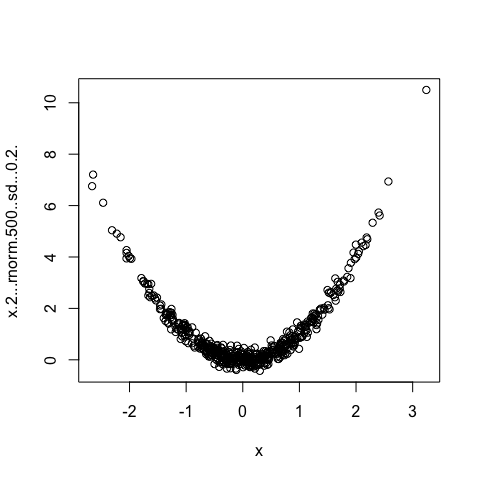
\includegraphics[width=\maxwidth]{figure/unnamed-chunk-2-1} \end{Schunk}
\caption{A distribution of observed values diameter increment values (gray bars). We assume (in this case I know it) that these values come from some true distribution (population or data-generating process) that I plotted here in dashed red color. If we would draw more and more data, the gray bars would approach the true distribution}
\label{fig: data distribution}
\end{center}
\end{figure}

Wie kann man nun die Eigenschaften der beobachteten Stichprobe zusammenfassen? Ein paar grundlegende Eigenschaften wären beispielsweise das Minimum und das Maximum, der Mittelwert, oder der Modalwert (die Maximalverteilung, d.h. der Wert der höchsten Beobachtungsdichte). Außerdem  gibt es zwei weitere Maßzahlen, die ebenso oft Gebrauch finden: Moment und Quantil.


Der Begriff 'Moment' mag vielleicht nicht jedem geläufig sein, aber vermutlich wurde schon einmal das erste und zweite Moment der Verteilung berechnet. Diese sind ebenfalls unter den Bezeichnungen Mittelwert und Standardabweichung bekannt. In general, das n-te moment $\mu_n$ of a distribution $f(x)$ around a value c is defined as 

\begin{equation}
\mu_n(c) = \int_{-\infty}^{\infty} f(x) (x - c)^n dx
\end{equation}

or, for a finite number of observations 

\begin{equation}
\mu_n(c) = \frac{1}{N}\sum_{i=1}^N (x_i - c)^n dx
\end{equation}

The first moment, with c=0, is simply the mean. For the following higher moments, it is common to consider the central moments, which are obtained by setting c to the mean, because their values are easier interpretable as indicators of the distribution's shape.\footnote{To estiamte the variance, we often replace the 1/N term by a bias-correction of 1/(N-1)} The 3 higher central moments are called the variance(n=2, identical to standard deviation squared, measure of spread), the skewness (n=3, measure of asymmetry in the distribution) and the kurtosis (n=4). 

Quantiles are the second central class of summary statistics for describing continous distributions. If we have a distribution such as the figure above, we can ask ourself: which is the value of the variable that divides the data in half, so that half of the observed data are lower, and half are higher than this value?\marginnote{Half of the data are lower, and half of the data are higher than the 0.5 quantile, which is called the median} This point is called the median, and also the 0.5 quantile. More general, the 0.x quantile is the value at which a fraction of 0.x of the data is smaller. 

\subsection{Correlation - summarizing the dependence between continous variables}

A second important case for summary statistics is correlation. Correlation methods measure the dependence between continous variables. Unfortunately, there are quite a number of measures of correlation, and it is imporant to distinguish between them. The two most important are:

\paragraph{Linear coefficients:}Linear coefficients, most notably the widely used "Pearson's correlation coefficient", measure the linear dependence between two variables. Pearson's correlation coefficient is widely used because it computes fast and is easily interpretable. However, it can be misleading if variables are not in a linear dependence. This effect is displayed in Fig.~\ref{fig: correlation}.

\paragraph{Rank correlation coefficients:} Rank correlation coefficients, such as ``Spearman's rank correlation coefficient'' and ``Kendall tau rank correlation coefficient'' measure how well the variables match in their tendency to increase or decrease, without considering the extend or linearity of this increase. They are preferable if you think variables could be in a nonlinear relationship.

\paragraph{Strong correlation != important effect:} Also visible in Fig.~\ref{fig: correlation} is an often misunderstood property of correlations and dependence - a high correlation coefficient does not mean that a variable has a strong reaction to another variable. All that is needed to obtain a high correlation coefficient is little spread around the line (see middle row - the effects are different, but the correlation is the same). 


\begin{figure}[htbp]
\begin{center}
\begin{Schunk}
\begin{Soutput}
Error in library(mvtnorm): there is no package called 'mvtnorm'
\end{Soutput}
\begin{Soutput}
Error: konnte Funktion "rmvnorm" nicht finden
\end{Soutput}
\begin{Soutput}
Error in RotNormal(200, c(0, pi/12, pi/6, pi/4, pi/2 - pi/6, pi/2 - pi/12, : konnte Funktion "rmvnorm" nicht finden
\end{Soutput}
\begin{Soutput}
Error in Others(800): konnte Funktion "rmvnorm" nicht finden
\end{Soutput}

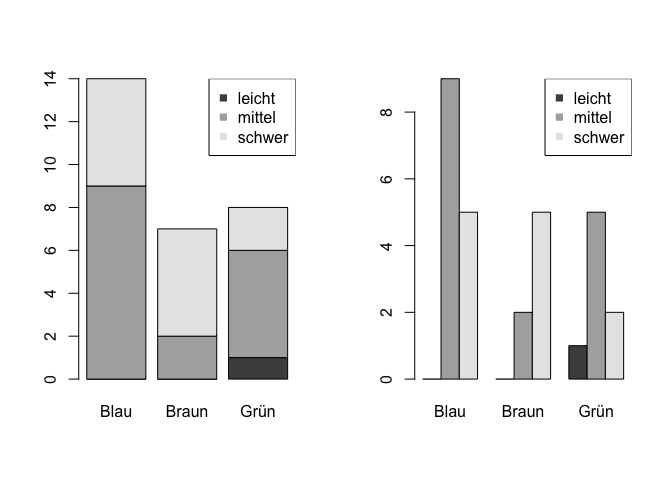
\includegraphics[width=\maxwidth]{figure/unnamed-chunk-3-1} \end{Schunk}
\caption{Demonstration of possible correlations with the Pearson's correlation coefficients. Note that many datasets that show a clear dependence between variables are assigned a Pearson's correlation coefficient of 0 because the dependence is not linear.}
\label{fig: correlation}
\end{center}
\end{figure}

\subsection{Contingency tables - summarizing disrecte outcomes of several variables}

Finally,\marginnote{This dataset from Berkeley is a famous example for the Simpson's paradox. Read up on wikipedia about this important statistical trap.} a classic concept for summarizing binary or categorical data are contingency tables. Here an example from a classical dataset available in R on aggregate data on applicants to graduate school at Berkeley for the six largest departments in 1973 classified by admission and sex. I show only the first department.

\begin{Schunk}
\begin{Sinput}
UCBAdmissions[,,1]
\end{Sinput}
\begin{Soutput}
          Gender
Admit      Male Female
  Admitted  512     89
  Rejected  313     19
\end{Soutput}
\end{Schunk}


\vspace{1cm}
\begin{fullwidth}
\begin{mdframed}
    
\textbf{In R:} 

For the various options to calculate descriptive statistics in R, see \href{http://www.uni-kiel.de/psychologie/rexrepos/rerDescriptive.html}{here}

\end{mdframed}
\end{fullwidth} 


\section{Visualization}

\marginnote{Type ?anscombe in R to see the code to create these plots and to calculate the statistical properties of the datastes}

Summary statistics are useful, but also dangerous. A famous example is Anscombe's Quartet, a hypothetical dataset of four observations that are identical in classical summary statistics such as mean, variance, correlation, regression line, etc. \citep{Anscombe-Graphsinstatistical-1973}. It is therefore very useful to get a graphical overview of your data, additionally to the summary statistics that you may calculate.

\begin{figure}[htbp]
\begin{center}
\begin{Schunk}

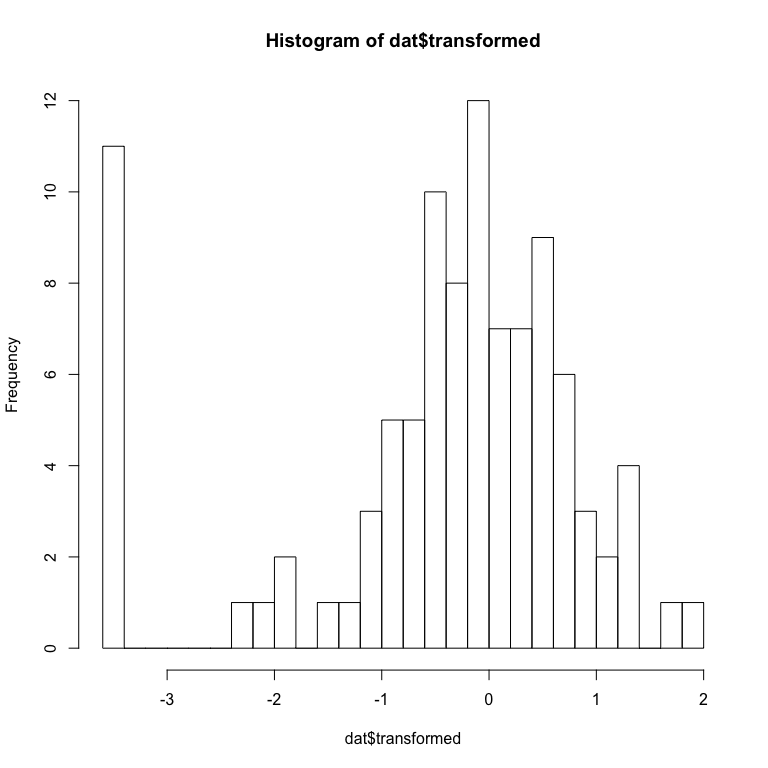
\includegraphics[width=\maxwidth]{figure/unnamed-chunk-5-1} \end{Schunk}
\caption{Anscombe's Quartet, a hypothetical dataset of four observations that are identical in classical summary statistics such as mean, variance, correlation, regression line, etc.}
\label{fig: Anscombes Quartet}
\end{center}
\end{figure}


\subsection{Principles of visualization}

The principle\marginnote{Examples of distorting graphics \href{https://en.wikipedia.org/wiki/Misleading_graph}{here}} of graphics and visualization is to represent the data as accessible and truthful as possible. The reader should get the best possible overview about the data in the shortest possible time. And, of course, the graphics should look nice as well. First of all, some general hints that may help:

\begin{itemize}
\item Simple is better than complicated
\item Avoid excessive color. Graphics should be b/w readable if possible (use a color gradient that is a gradient in intensity at the same time, use dashing of lines additional to colors). If your graphic relies on color, try to choose colors that can be read by color blinds (avoid red/green).
\item Truthfulness: avoid distortions. Use quadratic figures unless there are particular reasons. Axis should start at 0 unless you have good reasons not to. If presenting several graphics, use the same scale unless there are good reasons for it. 
\item Don't manipulate graphics by hand
\item Output in a vector format (pdf, eps, svg)
\end{itemize}

\begin{figure}[htbp]
\begin{center}

\setkeys{Gin}{width=\textwidth}
\begin{Schunk}

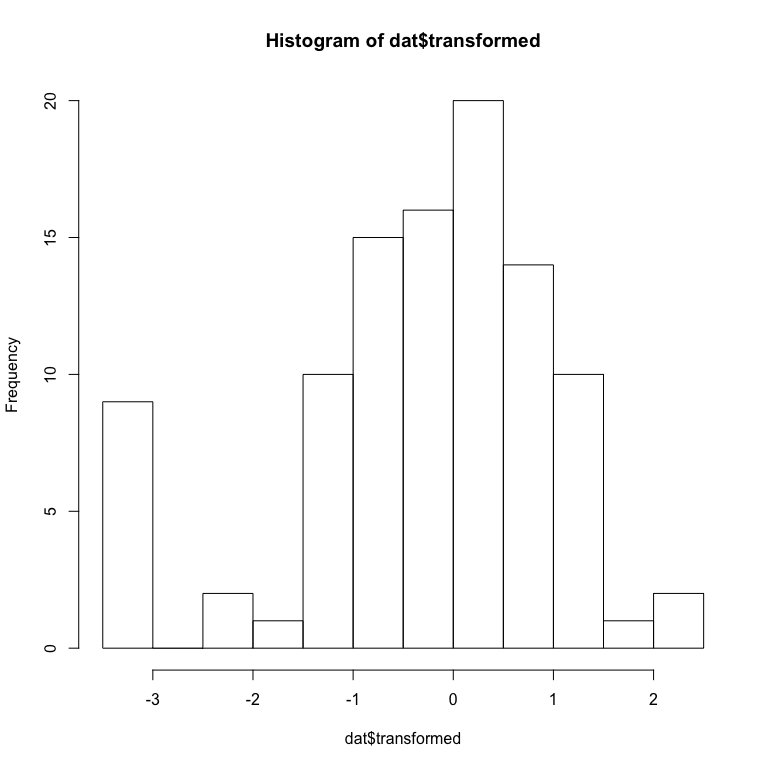
\includegraphics[width=\maxwidth]{figure/unnamed-chunk-6-1} \end{Schunk}
\caption{Four typical plot types, from top left to bottom right: a) A line plot to represent continous measurements of one variable; b) a scatter plot to represent the relationship between two continous variables; c) a bar plot to represent measurements in discrete groups / variables; d) a box plot to represent repeated continous measurements in discrete groups.}
\label{fig: exaple plots}
\end{center}
\end{figure}


\subsection{Graph types}

There is a large, nearly infinte number of possible visual representation of data. I provide here four very common graph types. 

\paragraph{Line plots:} Line plots are used to visualize continous, ordered measurements. Typical examples would be time series, continous variations of a parameter, or a mathematical function. Example in Fig.~\ref{fig: exaple plots}a.

\paragraph{Scatter plots:} Scatter plots show two continous continous variables that are measured in pairs. Typical example is when you have repeated measurements of several variables, and you want to see if they correlate. Example in Fig.~\ref{fig: exaple plots}b.

\paragraph{Bar plots:} Bar plots show an information (counts, or a continous variable) for discrete groups. Example in Fig.~\ref{fig: exaple plots}c.

\paragraph{Box plots:} Box plots are very common to show the distribution of a continous variable across several discrete groups. They typically consist of a box, whiskers (lines), and potentially points around the whiskers. What those means depends on the software used to create the plots, but the typical interpretation is that the box covers the central 50\%, with the median in indicated in the middle. The whiskers aim at providing an estimate of the range of your data, except for outliers. Of course, what is counted as an outlier depends on your assumptions. If you must know, the technical definition is that the whiskers are at the most distant observation less than or equal to the upper quartile plus 1.5 the length of the interquartile range. Example in Fig.~\ref{fig: exaple plots}d.

\vspace{1cm}
\begin{fullwidth}
\begin{mdframed}
    
\textbf{In R:} 

There are number of excellent introductions to graphics with R, so that I won't bother to provide details here. As a start, I recommend looking at \href{https://github.com/florianhartig/ResearchSkills/tree/master/Labs/Statistics/Practicals/GraphicsInR}{exercise on graphics with R} that accompanies this primer, as well as at 

\begin{itemize*}
  \item \href{http://www.statmethods.net/graphs/index.html}{QuickR}
  \item \href{http://shinyapps.org/apps/RGraphCompendium/index.php}{RGraphCompendium}
  \item \href{http://www.uni-kiel.de/psychologie/rexrepos/rerDiagrams.html}{rexrepos}
\end{itemize*}

\end{mdframed}
\end{fullwidth} 


\chapter{Inferential statistics}

\marginnote{Statistical inference is drawing conclusions from observations using statistical methods} 

Inferential statistics is concerned with inference, i.e. drawing conclusions from observations. An example of an inferential conclusion would be the following: we observe that 15 of 20 subjects that were administered a certain medication (treatment group) improved in their condition, while only 3 of 20 subjects that did not receive medication (control group) improved --> statistical inference: we can say with a certainty of X that the medication has a positive effect.  


\section{The data-generating model}

\marginnote{Statistical inference is not always, but in most cases, connected to the idea of a data-generating model}

A central concept for many methods in inferential statistics is the idea of the data-generating model. In a nutshell, the data-generating model comprises our fixed assumptions about how our observed data arises (normally distributed noise, linear response). We can then calculate (inference) the unkown quantities (difference between treatment and control) conditional on the our fixed assumptions 

\marginnote{In statistics, one often uses the word treatment to describe manipulations to experimental units. Here, the two types of music would be called treatments. The particular treatment of "doing nothing" is called the control.} 

Imagine we want to know whether plant growth can be affected by music. We might take two pots, each with a plant, and expose one to classical music and the other to heavy metal. Inevitably, one of them will grow taller, but this could be by chance, as there is always some variation in the growth rates. 

Hence, we need more repetitions. Let's say we take a few more pots, 30 in the hypothetical case I show below

\begin{figure}[htbp]
\begin{center}
\begin{Schunk}

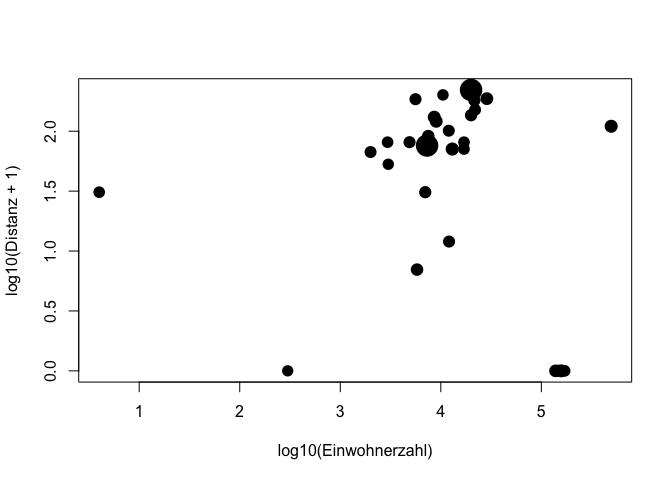
\includegraphics[width=\maxwidth]{figure/unnamed-chunk-7-1} \end{Schunk}
\caption{Groth measurements under three different treatments}
\label{fig: plant growth music}
\end{center}
\end{figure}

\marginnote{Remember the interpretation of the boxplots - the strong line in the middle is the median. The box covers the central 0.5 quantile of the distribution.}
There seem to be some differences between the three cases, but there is also quite a bit of variation in plant growth within each treatment (we have on average seven observations per treatment here). Hence, it is still possible that the differences that we observe have arisen by chance. 

If we want to say something definite about the probability of a difference between those two treatments and the control, we need to make a model that describes the stochastic variation in the data, which then allows us to calculate things such as the probability of the observed differences arising by chance. These assumptions are what we call a statistical model (eqivalent: stochastic process, data-generating model). \marginnote{A statistical model describes how the response variable arise as a functiono of the predictors as well as some random (stochastic) processes}. 

The more common class of models used for this purpose are parametric statistical models.\marginnote{Parametric statistics uses statistical models that describe the data-generating process in terms of functions and distributions that have parameters that then need to be fit} For the data that we have here, a parametric statistical model might, for example, make the assumptions that there is a mean growth rate for each treatment (control, classical and heavy metal), but that the growth of each individual plant varies with a normal distribution around the mean growth of its respective group. The parameters of this model are the unknown mean growth rates and the variance of the normal distribution. Those parameters are then fit to the data with methods explained in this chapter, and based on the fit one can calculate, for example, the probability that the data would arise if there was no difference between the groups.

The other option to obtain a data-generating model are non-parametric methods.\marginnote{non-parametric statistics tries to avoid making assumptions about the data-generating process. Typically, the data-generating process is emulated by using the data itself, e.g. by resampling methods.} Non-parametric methods bypass the necessity of making assumptions, e.g. about the distribution of the data, typically by randomizing or resampling the data itself. How does this work? For the plant growth, for example, we could answer the question of how likely it is to see the observed data if there is no difference between groups also without making an assumption about the distribution - we simply throw all observations in one pot, irrespective of their treatment, and then re-distribute them randomly on the three treatments. If we do this many times (e.g. 1000 times), we can get a good idea how likely it would be to obtain the observed differences if treatment has no effect. 

Non-parametric methods are an important branch of modern statistics. Their advantage is obviously that they don't make assumptions.\marginnote{The higher sensitivity of parametric methods relies on the fact that they make assumptions, which, in a sense, are like additional data. Of course, all results then rely on those assumptions being correct. We will talk about how to check parametric assumptions later in the chapter.} On the other hand, parametric methods are typically much faster, and if their assumptions are correct, they are more sensitive and powerful, meaning that, with the same amount of data, they are more likely to detect an effect if it is there. For the latter two reasons, parametric methods are currently the basis of most statistical analysis.


\section{Inferential outputs}

Based on the data-generating model (parametric or non-parametric), we can now apply different inferential procedures to draw conclusion about our data (in our case: to decide if music makes a difference or not). In standard statistics, there are two main inferential procedures that are applied in all kind of settings and models, and the outputs of these two procedures are: p-values and maximum likelihood estimates. A third procedure, the posterior calculated by Bayesian inference, has become more fashionable lately. I will mention it shortly at the end of this section 

\subsection{p-values}

The use of p-values is connected to the inferential method of null hypothesis significance testing (NHST). The idea is the following: if we have some data observed, and we have a statistical model, we can use this statistical model to specify a fixed hypothesis about how the data did arise. For the example with the plants and music, this hypothesis could be: music has no influence on plants, all differences we see are due to random variation between individuals. Such a scenario is called the null hypothesis. \marginnote{A null hypothesis $H_0$ is a fixed scenario that makes predictions about the expected probabilities of different observations.} Although it is very typical to use the assumption of no effect as null-hypothesis, note that it is really your choice, and you could use anything as null hypothesis, also the assumption: "classical music doubles the growth of plants". It's the analyst's choice what to fix as null hypothesis, which is part of the reason why you can choose among such a large number of available tests. We will see a few of them in the following chapter about important hypothesis tests.

If we have a null hypothesis, we calculate the probability that we would see the observed data or data more extreme under this scenario. This allows us to test whether our null hypothesis is compatible with the data, and thus called a hypothesis tests. We call the probability to see the data or more extreme the p-value. \marginnote{The p-value is the probability to see the data or more extreme data under the null-hypothesis.} 

\begin{equation}
p := p(d >= D_{obs} | H_0)
\end{equation}

If the p-value falls under a certain level (the significance level $\alpha$), we say we have significant evidence to reject the null hypothesis. The level of $\alpha$ is a convention, in ecology we chose typically 0.05, so if a p-value falls below 0.05, we can reject the null hypothesis. \marginnote{if p<0.05, we say we have significant evidence to reject the null-hypothesis.} 

A problem with hypothesis tests and p-values is that their results are notoriously misinterpreted. The p-value is NOT the probability that the null hypothesis is true, or the probability that the alternative hypothesis is false, although many authors have made the mistake of interpreting it like that \citep[][]{Cohen-earthisround-1994}. Rather, the idea of p-values is to control the rate of false positives (Type I error). When doing hypothesis tests on random data, with an $\alpha$ level of 0.05, one will get exactly 5\% false positives. Not more and not less.  

\subsection{Maximum likelihood estimation}

The second type of output that is reported by most statistical methods are maximum-likelihood parameter estimates. In a nutshell, the maximum-likelihood estimate (MLE) is our best estimate for the parameters in our model (e.g. a difference between the treatments and the control in our example). 

In a bit more detail: in statistics, we define the likelihood as a function of the model parameters $\theta$ as  

\begin{equation}
L(\theta) := p(dD_{obs} | M(\theta))
\end{equation}

, i.e. as the function that is obtained by calculating the probability of obtaining the observed data when we vary the model parameters.

The maximum-likelihood estimate (MLE)\marginnote{It is important to note that the MLE is the parameter set for which the data is most likely, not the most likely parameter set!} is then defined as the combination of parameters or model assumptions for which the likelihood is maximal. So, while the p-value is the probability of the observed data or more extreme data under a fixed (null) hypothesis, the MLE gives us the ``hypothesis'' that has the highest probability to produce the observed data  

The MLE is only a single parameter value.\marginnote{A point estimate is something like a single best estimate.} This type of estimate is often called a point estimate. However, a point estimate is typically of little use if we don't know how certain it is.\marginnote{Confidence intervals provide an estimate of uncertainty around the point estimate.} Therefore, parameter estimates are usually accompanied by confidence intervals. Sloppily you can think of the 95\% confidence interval of a parameter as the probable range for this area. Somewhat confusing for many, it's not the interval in which the true parameter lies with 95\% probability. Rather, in a repeated experiments, the standard 95\% CI will contain the true value in 95\% of all cases. It's a subtle, but important difference. However, for now, don't worry about it. The CI interval is roughly the range within which we expect the true parameter to be. 

\subsection{Bayesian inference}

To conclude\marginnote{Bayesian methods calculate a third quantity, the posterior probability. Although they can be used for any model, Bayesian methods tend to be used for more advanced statistics.} our overview on inferential products, one method is still lacking - Bayesian methods calculate a quantity that is called the posterior parameter estimate. It is similar, but not identical to the parameter estimates discussed previously. You won't need this here, but if you want to know more about those, have a look at \citep{Gelman-BayesianDataAnalysis-2003} and at my website \href{http://florianhartig.github.io/LearningBayes/}{Learning Bayes}.

\subsection{Different methods != different models}

You know now that there are three different things that statisticians typically calculate: p-values, MLE, and the posterior. For a given data-generating process, you can always calcuate any of the three.

I\marginnote{ANOVA , t-tests and linear regression are only different evaluations of the same model} make this point because many people wrongly assume that they use different models when they are indeed only using different ways to evaluate them. An example is the case of ANOVA, t-tests and linear regression. All of them are based on the same data-generating process - some fixed effects between groups and an iid normal observation error on top. ANOVA and t-tests specify different null-hypothesis, and the linear regression searches for the MLEs. You could additionally calculate the Bayesian posterior if you wanted.

\section{Important hypothesis tests}

After having discussed the basic statistical outputs, lets move to practice and get to know the two probably most applied hypothesis tests, the t-test and ANOVA. I told you already that they are based on the same data-generating process, but specify slightly different null-hypotheses. 

\subsection{t-test}

A t-test tests for differences between the means of two normally distributed samples; or if there is only one sample, between 0 and the mean of the sample.\marginnote{To stay in our previous classification, we would say the response variable in continuous, and the predictor is categorical (group 1 or group 2), or, if there is only one group, there is no predictor.} Again, the statistical model underlying is that of a normally distributed response, and the null hypothesis is that there is no difference in the mean of this normal distribution for the two groups, respectively that the sample mean is 0 if we have only one group. Also, depending on the software used, there are usually a number of adjustments possible, e.g. relaxing the assumption that the two groups have the same variance. Here, I show an example in R, using the classical data from \citet{Student-probableerrormean-1908}. The data show the effect of two soporific drugs (increase in hours of sleep compared to control) on 10 patients. 

\begin{figure}[htbp]
\begin{center}
\begin{Schunk}

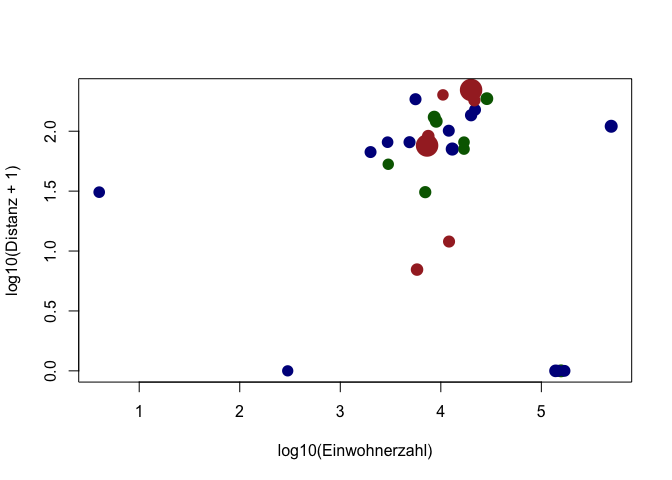
\includegraphics[width=\maxwidth]{figure/unnamed-chunk-8-1} \end{Schunk}
\caption{Data from \citet{Student-probableerrormean-1908}}
\label{fig: Student Sleep Data}
\end{center}
\end{figure}

\begin{Schunk}
\begin{Sinput}
## Traditional interface
with(sleep, t.test(sleep$extra[sleep$group == 1], extra[group == 2]))
\end{Sinput}
\end{Schunk}

\begin{Schunk}
\begin{Sinput}
## Formula interface
t.test(extra ~ group, data = sleep)
\end{Sinput}
\begin{Soutput}

	Welch Two Sample t-test

data:  extra by group
t = -1.8608, df = 17.776, p-value = 0.07939
alternative hypothesis: true difference in means is not equal to 0
95 percent confidence interval:
 -3.3654832  0.2054832
sample estimates:
mean in group 1 mean in group 2 
           0.75            2.33 
\end{Soutput}
\end{Schunk}

Note that the output provides a p-value (H0 = no difference), but also the maximum-likelihood estimate for the difference of the means, together with the confidence intervals. This is goes beyond the classical t-test, but probably the programmers assumed that you would also want to have the best estimate for the difference of the means.

Suggestion for reporting this result: p>0.05: differences between groups were not significant. p<0.05: we found a difference of X +- Confidence interval between the groups (p-value for difference from a t-test was X). 

\subsection{Analysis of variance (ANOVA)}

ANOVA or analysis of variance can mean different things to different people. The standard ANOVA makes basically the same assumptions as a t-test (normally distributed responses), but allows for more than two groups. More precisely, it tests if the measured response (i.e. the dependent variable) is influenced by one or several categorical variables that could have two or more levels could also interact. An interaction\marginnote{An interaction = one variable modifies the effect of another variable} between two variables means that the value of one explanatory variable affects how strongly another explanatory variable affects the response.

While the word ANOVA is generally associated with the assumption explained above (which correspond to a t-test / linear regression, see next chapter), the concept of ANOVA can be extended in the same way as linear regression models can be extended to generalized linear models etc. Hence, we can do ANOVA also for models with non-normally distributed errors (of course you have to tell this the software, it won't do it automatically). You therefore have to read carefully what people mean if they use the term.

Here a simple example with a standard ANOVA (normal errors), testing whether weight (of chicken) depends on their diet, where diet is a factor variable with four levels:

\begin{Schunk}
\begin{Sinput}
aovresult <- aov(weight~Diet, ChickWeight)
summary(aovresult)
\end{Sinput}
\begin{Soutput}
             Df  Sum Sq Mean Sq F value   Pr(>F)    
Diet          3  155863   51954   10.81 6.43e-07 ***
Residuals   574 2758693    4806                     
---
Signif. codes:  0 '***' 0.001 '**' 0.01 '*' 0.05 '.' 0.1 ' ' 1
\end{Soutput}
\end{Schunk}

We find a p-value of  6.43e-07, which is highly significant at an $\alpha$ level of 0.05. Hence, we can reject the null hypothesis that the diet has no influence on the response "weight". Note that in this case, we don't get any parameter estimates, and we can't say anything about which of the diets differs from which. If you want those, there are two options:

\begin{itemize}
\item Either you apply what is called post-hoc testing, which means that you test for differences (e.g. with a t-test) between the diets.
\item Or you switch to a regression, which is described in the next chapter
\end{itemize}

If you do post-hoc testing, you are doing multiple tests on the same data. This is a problem - the idea of the p-value is that you calculate the probability of seeing the data under ONE null hypothesis. If you do this, you will get at most 5\% error at an $\alpha$ level of 0.05. \marginnote{When doing multiple tests on the same data, we need to correct the p-values for multiple testing.} However, if we do multiple tests, we are testing multiple null hypotheses, and there are more options for the test statistics to get significant just by chance. Hence, we need to correct the p-values for multiple testing. There are a number of options to do so, google is your friend. 

\subsection{Other important tests}

t-test and ANOVA are the commonly needed tests in the context of the research skills module, but there are many more tests that could be potentially important. A list of tests that have wikipedia articles can be found at \href{http://en.wikipedia.org/wiki/Category:Statistical_tests}{here} 


\section{Regression}

As explained earlier, regression does not necessarily mean using a different statistical model as in hypothesis testing (ANOVA and the linear regression model in R use the same assumptions). However, the goal of regression is a different one. While hypothesis tests are all about seeing whether the data would be compatible with a null-hypothesis, regression is about finding the best-fitting hypothesis or parameters (the MLE). Hence, a regression model tries to find the parameter combination that produces the highest probability to create the observed data, given the model assumptions.

\subsection{Linear regression}

The most basic regression model is the linear regression. The assumption here is that we have a response that depends on the predictors in a form of 

\begin{equation} \label{eq: linear regression}
y \sim a \cdot x + b + \epsilon 
\end{equation}

where y is the response, x is a predictor, a is the parameter that fits how strongly the predictor influences the response, b is the intercept, and $\epsilon$ is the random variation, which in a linear regression is assumed to be normally distributed. 

In R, we can do such a regression by typing

\begin{Schunk}
\begin{Sinput}
fit = lm(airquality$Temp~airquality$Ozone)
summary(fit)
\end{Sinput}
\begin{Soutput}

Call:
lm(formula = airquality$Temp ~ airquality$Ozone)

Residuals:
    Min      1Q  Median      3Q     Max 
-22.147  -4.858   1.828   4.342  12.328 

Coefficients:
                 Estimate Std. Error t value Pr(>|t|)    
(Intercept)      69.41072    1.02971   67.41   <2e-16 ***
airquality$Ozone  0.20081    0.01928   10.42   <2e-16 ***
---
Signif. codes:  0 '***' 0.001 '**' 0.01 '*' 0.05 '.' 0.1 ' ' 1

Residual standard error: 6.819 on 114 degrees of freedom
  (37 observations deleted due to missingness)
Multiple R-squared:  0.4877,	Adjusted R-squared:  0.4832 
F-statistic: 108.5 on 1 and 114 DF,  p-value: < 2.2e-16
\end{Soutput}
\end{Schunk}

\begin{figure}[htbp]
\begin{center}
\begin{Schunk}

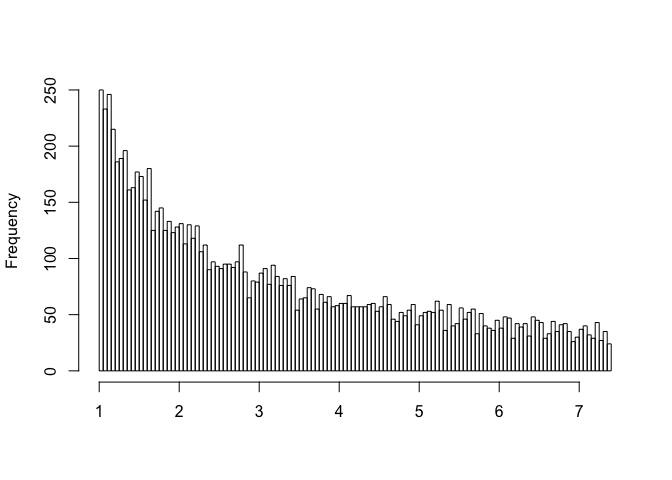
\includegraphics[width=\maxwidth]{figure/unnamed-chunk-13-1} \end{Schunk}
\caption{Airquality data: Temperature plotted against Ozone. Relationship indicated by the regression line.}
\label{fig: LR}
\end{center}
\end{figure}

You can use the same code regardless of whether your predictor is continuous or categorical. In case of continuous variable, a line is fit to the data. In case of a categorical variable with n levels, the first level is set as the reference (intercept), and n-1 parameters are fitted for the following levels that describe the difference to the reference. 

The fitted parameters appear in the column "Estimate". This tells us how much the predictor, in this case Ozone, affects the response, in this case the Temperature: for each unit of Ozone more, temperature increases by a 0.208 units, with a standard error (confidence interval) of 0.019. Apart from seeing how a regression output looks like, this teaches us another valuable lesson: the fact that we have used temperature as a response here and ozone as a predictor doesn't mean that ozone causally affects temperature. \marginnote{Correlation is not causality.} In fact, it is likely the other way around: if we have more sun, it's hotter, and we tend to have more ozone as well. Regression, as most other statistical analysis, doesn't establish causality, it establishes correlation. What we are saying is that if our ozone measurements go up, we can be pretty sure that it is hotter as well. Doesn't mean that ozone creates heat. Correlation is not causality. 

The regression results gives us a lot of p-values as well. These are results of various hypothesis tests that are performed automatically for you after the regression is done. For example, we get a p-value for each parameter. This p-value is based on a particular type of t-tests where the full model is tested against the model with the parameter set to 0. There is also other p-value, based on a different test statistics at the end of the regression output. This tests the null hypothesis that all parameters are zero.  


\vspace{1cm}
\begin{fullwidth}
\begin{mdframed}
    
\textbf{Specifying different model assumptions in R:} 

Response y depends linearly on a variable a (continous or categorical)

\begin{Schunk}
\begin{Sinput}
fit = lm(y~a)
summary(fit)
\end{Sinput}
\end{Schunk}

Response y depends linearly on two variables a and b (continous or categorical), but the value of either variable doesn't influence the effect the other variable has on the response (no interaction)

\begin{Schunk}
\begin{Sinput}
fit = lm(y~a+b)
summary(fit)
\end{Sinput}
\end{Schunk}

Response y depends linearly on two variables a and b (continous or categorical), but the value of one variable does influence the effect the other variable on the response (interaction)

\begin{Schunk}
\begin{Sinput}
fit = lm(y~a*b)
summary(fit)
\end{Sinput}
\end{Schunk}

Response y depends as in $a + a^2$ on a variable a (continous or categorical)

\begin{Schunk}
\begin{Sinput}
fit = lm(y~a + I(a^2))
summary(fit)
\end{Sinput}
\end{Schunk}

the I() notation means that the following expression is interpreted as a mathematical formula. 

\end{mdframed}
\end{fullwidth}


\subsection{Checking the assumptions}

Formally, we can fit any data with a linear model. However, as in any statistical inference procedure the results (i.e. parameter estimates, p-values) are conditional on the assumptions that we have made. Hence, the p-value we get is conditional on the assumption that the data is actually from a process that conforms to eq.~\ref{eq: linear regression}. If it doesn't the p-value could be completely wrong. Hence, we have to check whether those assumptions are actually met. 

So, what were the assumptions of a linear regression? One problem I often encounter is that students remember that the assumptions were normal distribution. Hence, they look at whether the response variable is normally distributed. However, if you look sharply at eq.~\ref{eq: linear regression}, you see that this was actually not the point. If we shift around the terms in eq.~\ref{eq: linear regression}, we see that what is actually supposed to be normally distributed is 

\begin{equation} \label{eq: linear regression}
y - (a \cdot x + b ) \sim \epsilon 
\end{equation}

i.e. the difference between the observed value and the model predictions. These differences are called the residuals, and, according to the assumptions of our model, they should be normally distributed. To see whether this is indeed the case, one should perform a number of checks. The most basic is to plot the residuals against the fitted value AND against all predictors in the model. The resulting plots allow to diagnose a number of possible problems (Fig.~\ref{fig: ResidualPatterns})

\begin{figure}[htbp]
\begin{center}
\begin{Schunk}

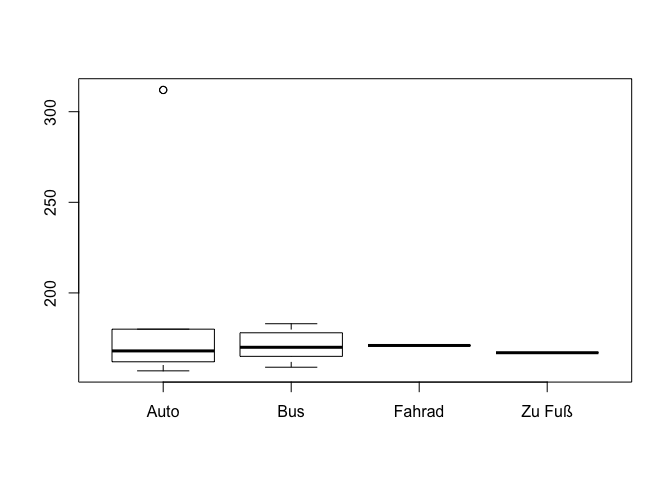
\includegraphics[width=\maxwidth]{figure/unnamed-chunk-18-1} \end{Schunk}
\caption{A collection of possible patterns when plotting the residuals against the fitted value (default in R) or a predictor.}
\label{fig: ResidualPatterns}
\end{center}
\end{figure}

Common problems and their solutions are 

\begin{itemize}
  \item Heteroskedasticity (variance changes) --> transform response, or use a regression model that can account for heteroscedasticity
  \item Pattern in the residuals --> Wrong functional form of the regression model. Try to add predictors, quadratic effects, interactions, or other things that change the functional form
  \item Distribution not normal --> Assuming this is not due to one of the earlier problems (no pattern / no heteroskedasticity), you can still try a variable transformation, or go to a regression with a different distributional assumption (see next section)
\end{itemize}  

There are further specialized plots to help with the diagnosis of these problems. You get then when applying the plot() command 


You get basic residual diagnostics by typing plot(fit), where fit is your fitted model object. For further details on residual diagnostics, see \href{http://www.statmethods.net/stats/rdiagnostics.html}{here}.



\section{Generalized linear regression models}

The general ideas of a linear regression was that 1) The response is continuous, theoretically from -infinity to + infinity, and 2) residuals are normally distributed around the model predictions. The idea of the GLM framework is take the linear regression framework is to allow you to work as before in the linear regression example, but relaxing both the assumptions about response values from - to + infinity, and the normality. To do this, we have to do two things

\begin{itemize}
  \item To get the output values on the range that we want, we wrap the linear model in a transformation function that forces the response on the right interval (typical intervals are positive, or between 0 and 1). This transformation is called the link function
  \item To fit other distributions, we have to tell the model to use something else than the Gaussian error function. 
\end{itemize}    
   
Let's talk about these points in a bit more detail.

\subsection{The link function}

We said above that a linear regression takes the form 

\begin{equation}
y \sim a \cdot x + b 
\end{equation}

That means that if x gets large, y could take any value, positive or negative. A trick to ensure that all predictions for y are positive, or within a certain range is using a link function of the form 

\begin{equation}
y \sim f^{link}(a \cdot x + b )
\end{equation}

Any function is possible, but as we see later typical choices are the exponential function, which ensures positives outcomes, and the inverse logit, which ensures are range between 0 and 1.

\subsection{Other distributions}

Well, this is conceptually the easy part, but maybe you are not yet aware what kind of distributions exist beside the normal. Two typical choices that we use below are the binomial (the distribution for coin flipping), and the Poisson distribution (a discrete probability distribution). There are many other choices available. Maybe it becomes more clear when we move to the actual examples in the next sections. 

\subsection{0/1 data - logistic regression}

Logistic regression is the most common analysis for binary data (presence/absence; survived/dead; infected/not infected). Logistic regression assumes that the distribution is binomial (coin flip model). To get the linear predictor on a scale between 0 and 1 that is necessary for the binomial distribution, we use the logistic link function (or inverse logit). 

evspace{1cm}
\begin{fullwidth}
\begin{mdframed}
    
\textbf{In R:} 

Here an example with the data of the Titanic survivors. Note that if you tell R to use the binomial distribution, the logit link is automatically selected. If you wanted, you could overrule this choice. 

\begin{Schunk}
\begin{Sinput}
library(effects)
\end{Sinput}
\begin{Soutput}
Error in library(effects): there is no package called 'effects'
\end{Soutput}
\begin{Sinput}
fmt <- glm(survived ~ age + I(age^2) + I(age^3), family=binomial, data = TitanicSurvival)
\end{Sinput}
\begin{Soutput}
Error in is.data.frame(data): Objekt 'TitanicSurvival' nicht gefunden
\end{Soutput}
\begin{Sinput}
summary(fmt)
\end{Sinput}
\begin{Soutput}
Error in summary(fmt): Objekt 'fmt' nicht gefunden
\end{Soutput}
\end{Schunk}

\end{mdframed}
\end{fullwidth} 




\subsection{count data - poisson regression}

Poisson regression is the standard choice for working with count data, although there are a few other options available as well. In poisson regression, the standard choice is to use a exponential function to make all values positive. The inverse of the exponential is the log, so we call this the log link. As before, R is choosing this automatically if you specify the distribution to be poisson. 

\vspace{1cm}
\begin{fullwidth}
\begin{mdframed}
    
\textbf{In R:} 

An example, using some data on the feeding of bird nestlings, in relation to their attractiveness:
\begin{Schunk}
\begin{Sinput}
schnaepper <- read.csv("schnaepper.txt", sep="")
fm <- glm(stuecke ~ attrakt, family=poisson, data = schnaepper)
summary(fm)
\end{Sinput}
\begin{Soutput}

Call:
glm(formula = stuecke ~ attrakt, family = poisson, data = schnaepper)

Deviance Residuals: 
     Min        1Q    Median        3Q       Max  
-1.55377  -0.72834   0.03699   0.59093   1.54584  

Coefficients:
            Estimate Std. Error z value Pr(>|z|)    
(Intercept)  1.47459    0.19443   7.584 3.34e-14 ***
attrakt      0.14794    0.05437   2.721  0.00651 ** 
---
Signif. codes:  0 '***' 0.001 '**' 0.01 '*' 0.05 '.' 0.1 ' ' 1

(Dispersion parameter for poisson family taken to be 1)

    Null deviance: 25.829  on 24  degrees of freedom
Residual deviance: 18.320  on 23  degrees of freedom
AIC: 115.42

Number of Fisher Scoring iterations: 4
\end{Soutput}
\end{Schunk}

\end{mdframed}
\end{fullwidth} 


\subsection{Residual checks in GLMs}

Residuals in glms are not supposed to be normally distributed, so don't use standard checks for normality such as normal qq plots to check for the appropriateness of the residuals. For not too complicate models, a good way to deal with this problem is to use the so-called pearsons residuals, which scale the observed differences between model and data by the expected variance of the model \footnote{in R, you can specify the option pearson in many fuctions, including the residual() function that you can apply to a fitted object}

One standard concern in poisson or binomial glms is that the variance of the poisson and binomial distribution cannot be adjusted, but is fixed by the mean. This is a problem you don't encounter in the normal linear model, because here the random part is modelled by a normal distribution, which has a parameter for the variance. A problem that appears very frequently in Poisson or binomial glms is overdispersion, i.e. that the residuals show more variance than expected under the fitted model. \marginnote{You can check for overdispersion by looking at the fitted deviance, or apply an overdispersion test} The easiest way to correct for this is to use the quasi-Poisson and quasi-binomial models available in the glm function. These models fit an additional parameter that modifies the variance of the Poisson and binomial glm. 


\chapter{Predictive statistics - machine learning}

A third class of statistical procedures that have become very important in recent years are predictive methods, often called machine-learning algorithms. The basic goal of this methods is to to be able to make predictions from a given dataset with the lowest possible error. In doing so, they typically use relatively complicated, often non-parametric methods that typically don't allow to calculate inferential products such as the MLE or p-values.

There is considerable tension between the more classical field of inferential statistics and the more modern field of machine-learning. For classical, inferential statisticians, machine learning methods have abandoned the idea of "learning from data", in the sense of comparing hypotheses to data, in favor of simply making predictions. A statistician concentrating on machine-learning would reply that in many applied problems, there is nothing to learn \footnote{Typical machine learning applications include predicting the interests of customers in web shops, the association of feature-rich satelite data with ground signals, or speech / face recognition. Machine-learning experts are currently sought-after by technology companies such as google, facebook and so on.}. The goal is to build an algorithm that is able to correctly predict given a complex dataset. The distinction between the goals of inferential statistics and predictive statistics, as well as the tension between these fields, are nicely summarized in the abstract of the extrememly recommendable article "Statistical Modeling: The Two Cultures" by \citet{Breiman-StatisticalModelingTwo-2001}:

\begin{quote}
There are two cultures in the use of statistical modeling to reach conclusions from data. One assumes that the data are generated bya given stochastic data model. The other uses algorithmic models and treats the data mechanism as unknown. The statistical community has been committed to the almost exclusive use of data models. This commitment has led to irrelevant theory, questionable conclusions, and has kept statisticians from working on a large range of interesting current problems. Algorithmic modeling, both in theory and practice, has developed rapidly in fields outside statistics. It can be used both on large complex data sets and as a more accurate and informative alternative to data modeling on smaller data sets. If our goal as a field is to use data to solve problems, then we need to move awayfrom exclusive dependence on data models and adopt a more diverse set of tools.
\end{quote}


I have included this short chapter because of the importance of predictive methods in modern statistics. A detailed explanation of the methods of machine-learning, however, is beyond this introduction. If you are interested in starting to learn more about predictive methods, I would recommend to start with the textbook by  \citet{James-IntroductiontoStatistical-2013} that I also recommend at the end of this primer for further reading. 

\chapter{Design of experiments}\label{cha: design of experiments}

Let's come back to one of the first point in this script: the data. If we have to collect data ourselves, we have to answer a number of questions. Which variables should we collect? At which values of those variables should we collect data? And how many replicates do we need?


\section{Selection of variables}

In a practical setting, we are typically interested in how a response is affected by a number of predictor variables. Clearly, we need to measure both response and this predictors of interest across a few of those predictor values to say something about the effect of the predictors. \marginnote{Correlation is not causality. For suggesting causality, we have to exclude confounding effects.} If we only wanted to know whether there is a correlation between predictors and response, our list of variables would be complete at this point. However, typically, we want to know not only if there is a correlation, but also whether we can say with some confidence that this correlation is causal. If we want to make this claim, we have to exclude that there are counfounding factors, also called confounding variables. 

\subsection{What is a confounding variable?}

Imagine we are interested in a response A, and we have hypothesized that A~B. Imagine there is a second predictor variable C that has an influence on A, but in which we are not interested in for the purpose of the question under consideration. Such a variable that is not of interest for the question is also called "extraneous variables". \marginnote{An extraneous variable is a variable that can influence the response, but is not of interest for the experimenter}. So we also have A~C, but we are not interested in this relationship. If we now take data, and don't measure C, it's usually not a bit problem as long as C is uncorrelated with B - it might create a bit more variability in the response, but by and large the effect of C should average out and we should still be able to detect the effect of B.

\begin{figure}[]
\begin{center}
\includegraphics[width = 6cm]{Confounding}
\caption{Diagram illustrating a confounding variable. A key requirement for being a counfounder is that the variable correlates both with the repsonse, and with the predictor variables that form our original hypothesis. If the second link is not there, the variable is not confounding and can be disregarded.}
\label{fig: Confounding}
\end{center}
\end{figure}

The problem of confounding appears when the extraneous variable C is for some reason correlated with the predictor variable of interest B. \marginnote{A confounding variable is an extraneous variable that correlated to both the response and a predictor variable of interest.} In that case, if we only measure B, we see both the effect of B and C. In this case, we may attribute the effect of C on A wrongly to the effect of B on A. \marginnote{A spurious correlation is a correlation that is caused by a confounding variable.} A correlation that is caused by an unmeasured confounding variable is called a spurious correlation.  

\subsection{What do do about confounding variables}

If we think there is a factor that could be confounding, we basically have three options

\begin{enumerate}
\item Best: control the value of these factors. Either fix the value (preferred if we are not interested in this factor), else vary the value in a controlled way (see below).
\item Second best: randomize and measure them
\item Third best: only randomize or only measure them
\end{enumerate}

Randomization means that we try to ensure that the confounding factor is not systematically correlated with the variable of interest (but can still cause problems with interactions and nonlinear relationships).


Measuring\marginnote{Variables that we include but that are not interesting to us are often called nuisance variables.} allows us to account for the effect in a statistical analysis, but cost power (see below) and, and we can't measure everything.

\section{Definition and bias of variables}

A common mistake at this step of the design is to take the variable definition and measurements for granted, and continue with considering the selection of replicates and so on. The step that is missing is to think about the following two questions. \marginnote{The consideration of these two questions is often referred to as construct validity, see also main RS script.}

\begin{enumerate}
  \item Do my variables measure what I want to measure
  \item What is the expected statistical (stochastic) error in my measurements, and what is the possible systematic error in my measurements
\end{enumerate}

\begin{figure}[]
\begin{center}
\includegraphics[width = 10cm]{RandomizedBlockDesign}
\caption{Illustrationo of a randomized block design, the probably most widely used desing on (observational) experiments to randomize the effect of unknown and unmeasured confounding variables. The idea of this design is that the unknown variables are likely correlated in space. By blocking all experimentally changing variables together, we avoid that they can become confounded iwth the unkonwn spatial variables.}
\label{fig: RandomizedBlockDesign}
\end{center}
\end{figure}


The first item may seem a bit odd, because one would think that we know what we measure. However, in many cases in ecological statistics and beyond, we do not measure directly the variable that we are interested in, but rather a proxy. So, for example, we want temperature on the plot, and we use temperature from a weather station 5 km away. Or, we want to look at functional diversity, but how can we exactly express this in terms of variables that we measure in the field.

The second questions relates to considering how much two measurements would differ if we do them repeatedly (stochastic),\marginnote{See main RS skript for more info on biases.} and how much measurements could be off systematically (e.g. because a method or instrument is systematically wrong, or because humans show particular biases).


\section{Selection of values for the independent (predictor) variables}

If we have decided which variables to measure / vary, we have to decide for the values at which we want to measure them. 

In\marginnote{The experimental unit is the entity that can be assigned a particular variable combination (e.g. treatment or control). Example: an individual plant, or a pot.} an experimental study, we usually vary variables systematically for a particular entity, e.g. a plant, a pot or a plot. This entity is called the experimental unit. Also observational studies have experimental units (the entities for which measurements are taken), but it usually not possible to completely control the variables. However, one usually has the option to make particular selections. Also in observational studies, it is key to ensure sufficient sufficient variation of the predictor variables across the experimental units to allow a meaningfull statstical analysis.

Here are a few points to consider

\subsection{Vary all variables independently}

A common problem in practice is that we have two variables,  but their values change in a correlated way. Imagine we test for the presence of a species, but we have only warm dry and cold wet sites. We say the two variables a collinear. In this case we don't know whether any observed effect is due to temperature or water availability. The bottom-line: if you want to separate two effects, the correlation between them must not be perfect - ideally, it would be zero, or failing that, as low as possible. 

\subsection{Interactions}

To be able to detect interactions between variables, it's not enough to vary all, you also need to have certain combinations. The buzzword here is (fractional) factorial designs. Google will help you.

\subsection{Nonlinear effects}

The connection of two points is a line. If you want to see whether the response to a variable is nonlinear, you therefore need more than two values of each variable.  


\section{How many replicates?}

We said before that the significance level $\alpha$ is the probability of finding false positives. This is called the type I error. There is another error we can make: failing to find significance for a true effect. This is called the type II error, and the probability of finding an effect is called power. \marginnote{Power is the probability of finding significance for an effect if it's there}. For standard statistical methods, power can be calculated. You have to look it up for your particular method, but in general assume that 

\begin{enumerate}
\item Power goes up with increasing effect size
\item Power goes down with increasing variability in the response
\end{enumerate}

This means that, unlike for the type I error which is fixed, calculation of power requires knowledge about the expected effect and the variability. This sounds really bad, but in most cases you can estimate from previous experience how much variation there will be, and in most cases you also know how big the effect has to be at least to be interesting. Based on that, you can then calculate how many samples you need.

\newpage
\begin{mdframed}
    
\textbf{Checklist experimental design}

\begin{description}

\item[( )] Clear, logically consistent question? Write it down. Read chapter about valid / good scientific questions in the lecture notes

\item[( )] Make sure you have read and considered all the issues of validity discussed in the main lecture notes. Go through the checklist validity at the end of the section in the main lecture notes.

\item[( )] Draft a design

  \begin{description}

  \item[( )] Vary the variables that you need to measure to answer your questions. Decide if you are intested in main linear effects, or also nonlinear effects or interactions. 
  
  \item[( )] Write down potential confounding variables. Decide if they are better controlled, randomised or measured? Are you sure they are confounding (correlated to response AND one or several of the predictors)
  
  \item[( )] Define the statistical hypothesis to be tested, including confounders. Write it down, as in $height  \sim age + soil * precipitation + precipitation^2$. 
  
  \item[( )] Choose how the variables will be varied in the experiment. Consider using software for this, e.g. for fractional factorial designs (in observational studies, you sometimes have limited control, but you can maybe estimate what variable combinations you will observe).
  
  \item[( )] Blocking - try to group different treatments / most different variable combinations together. The aim is that unknown / unmeasured variables are not correlated with your experimental variables (see pseudo-replication)
  
  \item[( )] Decide on the number of replicates. Make a guess for effect size and variability of the data, and either calculate or guess the number of replicates necessary to get sufficient power. What sufficient means depends on the field, but I would say you want to have a good chance to see an effect if it's there, so a power of $>80\%$ would be good. 
  
  \end{description}
  
\item[( )] Check design
  
  \begin{description}
  
  \item[( )] Play through the processes of collecting your data: simulate it in your mind or in R, make up some data, write it down. Everything seems OK?
  
  \item[( )] Play through the process of analysing your data. Which method? Can you answer your question? Do a power analysis!

  \end{description}


\item[( )] Revise if neccessary

\end{description}

\end{mdframed}


\chapter{Good to knows and further reading}

\section{Reproducibility and good scientific practice}

Reproducibility means that each step of your analysis is repeatable. Experience shows that it is not as trivial as it sounds to ensure reproducibility. Here some hints for making your data analysis reproducible

\begin{itemize}

\item{Once you have your raw data produced, NEVER change it. Store it in a save location, make a backup, and never touch it again}

\item{Typically you will have to do some cleaning, renaming etc. before the data analysis. If possible at all, make this through a script (e.g. R, python, perl). Store the script with the analysis.}

\item{Use a version control system for your code, and note for each output the revision number that the output was produced with.} \marginnote{See our RS lab on this topic \href{https://github.com/florianhartig/ResearchSkills/tree/master/Labs/VersionControl}{here}}

\item{When running the analysis, store the random seed and the settings of your computer to ensure reproducibility. In R, the easiest way to do this is to set the random seed by random.seed(123), and store the results of sessionInfo() which provides you with the version numbers of all the packages that you use}

\item{Think about running your code within an reporting environment such as Rmd or sweave}\marginnote{See our RS lab on this topic \href{https://github.com/florianhartig/ResearchSkills/tree/master/Labs/Statistics/reporting}{here}}


%\footnote{See also the R task view on \href{https://cran.r-project.org/web/views/ReproducibleResearch.html}{reproducible research}

\end{itemize}

\section{How to learn more about statistics}\label{sec: further readings}


\begin{itemize}

\item To complete this primer, I would recommend that you go through the \href{https://github.com/florianhartig/ResearchSkills/tree/master/Labs/Statistics}{practicals for this script}.

\item If you want one further practical textbook for beginners, I recommend \citet{Dormann-ParametrischeStatistik-2013} for German speakers (ebook free of charge for students from Freiburg, contact me) and \citet{Gotelli-PrimerEcologicalStatistics-2004} for English speakers. 

\item For the technically slightly more ambitious (it's still very elementary), I recommend \citet{James-IntroductiontoStatistical-2013}. You can download the pdf for free, and there is a MOOC available for the book with lectures and exercises. 

\item For more help and references, see the stats help website of our department  \href{http://biometry.github.io/APES/}{here}, in particular the recommendations regarding R scripts and statistics textbooks. 

\end{itemize}


\bibliographystyle{chicago}
\bibliography{/Users/Florian/Home/Bibliography/Databases/flo}


\addtocontents{toc}{\protect\setcounter{tocdepth}{0}}

\begin{appendices}

\chapter{R and Rstudio}

R itself is a command line program, meaning that you communicate with it through written commands in the R console. So, in principle, you could write your R code in an editor (even Microsoft Word), and the paste it in the R console. 

For the daily work, however, this is not very convenient, and we would like to have a program that combines the core R console, and editor, and maybe some other options like the option to display R graphical outputs, read in data, and so on. 

R comes with a simple editor that provides basic functionalities of that sort (note it looks a bit different on a Mac than the windows version we show here). This editor is called the RGui. To start the RGui, start the program R from your programs in Windows. Hava a look at the window popping up, and type 2+2 in the main window. After hitting enter you will end up with this:

\begin{figure}[]
\begin{center}
\includegraphics[width = 6cm]{rgui1.png}
\caption{Typing a simple calculation into the RGui}
\label{fig: Rgui1}
\end{center}
\end{figure}


The window you see here is called the R Console. Through the console, you interact with the core R program that does all the communcation. 

Let's write something else: R has a few standard datasets that are automatically loaded. We will be using the airmiles dataset, which shows the number of airmiles awarded over time. Let's shortly demonstrate how to do a plot with this dataset. Type:

\begin{Schunk}
\begin{Sinput}
plot(airmiles, col = 4)
\end{Sinput}
\end{Schunk}

The result should look like Fig.~\ref{fig: Rgui2}:

\begin{figure}[]
\begin{center}
\includegraphics[width = 6cm]{rgui2.png}
\caption{A figure produced with the RGui}
\label{fig: Rgui2}
\end{center}
\end{figure}

So, as you see, this apparently opens a new window (a graphics output) and plots airmiles against time. We'll discuss why and how this works. Before you get too used the the RGui, however, let's first move to RStudio, an alternative program to interact with R.

\section{The Rstudio editor}
 
RStudio basically offers the same functions as the RGui, but a many things can be done easier or are handled more comfortable for you. This is how it looks like:

\begin{figure}[]
\begin{center}
\includegraphics[width = 9cm]{rst_interface.png}
\caption{The RStudio editor, arguably the most popular editor for R}
\label{fig: Rstudio}
\end{center}
\end{figure}


\paragraph{Console:} The console that we have already seen is in the bottom-left panel. You can confirm that it behaves in the same way by typing in the same commands as we did before, i.e. 2+2, or plot the graph.

\paragraph{Editor:} Above the console (top left), r script files are displayed and can be changed in the editor. The idea of a script file is that you collect all the commands that you send to the console in one file, so that you can re-run it later.  

A typical script may look like that:

\begin{Schunk}
\begin{Sinput}
# the hash means this is treated as a comment
# this file is written by FH, 25.10.13

rm(list=ls(all=TRUE))  # this command means all variables in the memory are erase

# load some data

# do some plots
\end{Sinput}
\end{Schunk}

To send a part of the script to the console, you can use the run button on the top right border of the editor window. For everything we do from now on, I would strongly recommend writing in the script, and then sending it to console from there. 

\chapter{Handling data in R}
\label{HandlingDataInR}

\section{Variables}

Who has ever worked with a programming language? In a programming language, data is stored in variables / objects. This is how we assign the word "test" to the variable "VariableX"

\begin{Schunk}
\begin{Sinput}
VariableX = "test"
\end{Sinput}
\end{Schunk}

I can now access the variable by typing its name in the console, and it will return the value that it stores.
\begin{Schunk}
\begin{Sinput}
VariableX
\end{Sinput}
\begin{Soutput}
[1] "test"
\end{Soutput}
\end{Schunk}

We can see all the variables that we have specified in the global environment or R in the top-right corner or RStudio. You see that we have here the variable "VariableX" together with it's value. 


\begin{figure}[]
\begin{center}
\includegraphics[width = 6cm]{rst_globenv.png}
\caption{The global environment is displayed in the upper right corner of the The RStudio editor.}
\label{fig: Rstudio}
\end{center}
\end{figure}

\section{Data types and structures}

A variable can store different things: a number, a word, a list, or a whole dataset. 

The most simple case are variables that contain a **single value** only. Here, the only question is what kind of values the variable contains. The different data types a single value can have are called the **atomic types** - think of it as the basic data types in R. Important atomic types are: 

- boolean (TRUE / FALSE)
- integer (1, 2, 3, 5)
- numeric (1.1, 2.5, 3.456)
- factor ("red", "green", "blue")
- character ("a word", "another word")

If we have a collection of several atomic types, we speak of a data structure or an object (there is a difference but it doesn't matter here). Important examples of this are: 

- **vector** (a row of the same atomic types, e.g. [1,2,3,4,5] )
- **list** (basically like a vector, but can contain different types such as [1, "red", FALSE] )
- **data.frame** (a list of vectors, this is the standard format for data in R. Think of it as a spreadsheet - each colum is a vector and can have a different type)

A full list of data types is here http://www.statmethods.net/input/datatypes.html 
 
\subsection{Checking data types and structures}

Especially after reading in your data, it is important to check which type it has. The functions in R react differently depending on which atomic type you supply. 

If you want to see which type or structure a variable has, use the str command:

\begin{Schunk}
\begin{Sinput}
str(object)
\end{Sinput}
\end{Schunk}

To get a summary of your structure (e.g. mean per column, but what exactly is summarized depends on the data structure and type), use:

\begin{Schunk}
\begin{Sinput}
summary(object)
\end{Sinput}
\end{Schunk}

To try to make an automatic plot (R will choose what it thinks most suitable for this structure / type), type:

\begin{Schunk}
\begin{Sinput}
plot(object)
\end{Sinput}
\end{Schunk}

Try this with the object airquality. 

\subsection{Accessing columns, rows and elements in a data.frame or matrix}

As said, the most common structure in R is the data frame. Basically, columns are stored as a list of vectors, so that each column can be a different data type.

You can select columns in a number of ways:

- By name:
\begin{Schunk}
\begin{Sinput}
airquality$Ozone
\end{Sinput}
\end{Schunk}

- By column index: 

\begin{Schunk}
\begin{Sinput}
airquality[,1]
\end{Sinput}
\end{Schunk}

Note that here [,1] means the first column. You could get the first row by [1,].

\section{Selecting data}

The last type of accessing is an example of slizing. Slizing is a very powerfull technique that is available in most scientific programming languages. What it means is that you can access your data by typing in colums, rows, or particular elements. Look at the following commands (explanation always below):

\begin{Schunk}
\begin{Sinput}
airquality[,1:2]
\end{Sinput}
\end{Schunk}

gets the first colums 1 and 2.


\begin{Schunk}
\begin{Sinput}
airquality[4:6,1]]
\end{Sinput}
\end{Schunk}

gets rows 4 to 6 in column 1


\begin{Schunk}
\begin{Sinput}
airquality[c(1,2,3,4,7,8),1]
\end{Sinput}
\end{Schunk}

gets rows 1,2,3,4,7,8 in column 1. 

You see, we can select any combination of elemets we want very conveniently from the data frame. Even more convenient is how we can create selections.


\begin{Schunk}
\begin{Sinput}
1:10
\end{Sinput}
\end{Schunk}

gives us the values of 1 to 10

\begin{Schunk}
\begin{Sinput}
c(1,5,6)
\end{Sinput}
\end{Schunk}

the c() function combines values in one vector (it is neccessary to have the values in one vector for slicing)

\begin{Schunk}
\begin{Sinput}
c(1,5,6)
\end{Sinput}
\end{Schunk}

But we can also create selections with logical operators

\begin{Schunk}
\begin{Sinput}
airquality$Temp > 80
\end{Sinput}
\end{Schunk}

creates a vector with True on all temperature values that are > 80. I can store this and use it for selection, or use it immediately



\begin{Schunk}
\begin{Sinput}
airquality[airquality$Temp > 80 , ]
\end{Sinput}
\end{Schunk}

selects all rows with temperature > 80.


\section{loading data into R}

So far, we had the data already in the R program. Now, we will demonstrate how to load some data (we will use the airquality.txt file provided to you)

There are basically two options to load data

- with RStudio (point and click) - go to Environment (top right), import dataset, and follow instructions

- from the script with the read.table() command

The latter works like that


\begin{Schunk}
\begin{Sinput}
data = read.table("airquality.txt", header = T)
\end{Sinput}
\end{Schunk}

In this case it works nice because I have prepared the data in the most easy way. If you have other data formates (commas, semicolons, header / no header), consult the help of teh read.table command. See also http://www.statmethods.net/input/importingdata.html for more options, e.g. excel or database import. 

\subsection{Checking the data}

After loading the data, always check whether the data format is correct 

\begin{Schunk}
\begin{Sinput}
str(data)
\end{Sinput}
\begin{Soutput}
function (..., list = character(), package = NULL, lib.loc = NULL, 
    verbose = getOption("verbose"), envir = .GlobalEnv)  
\end{Soutput}
\end{Schunk}

You see here the atomic type of every column. Make sure it corresponds to what you want (sometimes numeric is read in as factor, or *vice versa*). If a column would have the wrong type, we have to change this by typing

\begin{Schunk}
\begin{Sinput}
as.factor(x)
\end{Sinput}
\end{Schunk}
or 
\begin{Schunk}
\begin{Sinput}
as.numeric(x)
\end{Sinput}
\end{Schunk}


Note: this data file is already included in R, so if you don't manage to load it, you can continue anyway. 

\chapter{Plot commands in R}

Before that, a few important references 

\begin{itemize}
\item \href{http://rgraphgallery.blogspot.de/search/label/3%20vartiable%20plots}{here}
\item Excellent: the \href{http://shiny.stat.ubc.ca/r-graph-catalog/#}{R Graph Catalog}
\item \href{http://rgm3.lab.nig.ac.jp/RGM/R_image_list?page=2282&init=true}{R Graphical Manual}
\item \href{http://www.statmethods.net/graphs/line.html}{QuickR}
\end{itemize}


\marginnote{An overview or R colors \href{here}{http://research.stowers-institute.org/efg/R/Color/Chart/ }}

\begin{Schunk}
\begin{Sinput}
plot(airquality$Ozone, airquality$Temp)
\end{Sinput}


{\centering \includegraphics[width=\maxwidth]{figure/unnamed-chunk-42-1} 

}

\end{Schunk}


\begin{Schunk}
\begin{Sinput}
hist(airquality$Ozone, breaks = 30, col = "darkred", xlab = "Ozone ")
\end{Sinput}


{\centering \includegraphics[width=\maxwidth]{figure/unnamed-chunk-43-1} 

}

\end{Schunk}


\begin{Schunk}
\begin{Sinput}
plot(airquality)
\end{Sinput}


{\centering \includegraphics[width=\maxwidth]{figure/unnamed-chunk-44-1} 

}

\end{Schunk}

pairs(airquality)


Simple Bar Plot 

\begin{Schunk}
\begin{Sinput}
counts <- table(mtcars$gear)
barplot(counts, main="Car Distribution", 
   xlab="Number of Gears")
\end{Sinput}


{\centering \includegraphics[width=\maxwidth]{figure/unnamed-chunk-45-1} 

}

\end{Schunk}

Grouped Bar Plot

\begin{Schunk}
\begin{Sinput}
counts <- table(mtcars$vs, mtcars$gear)
barplot(counts, main="Car Distribution by Gears and VS",
  xlab="Number of Gears", col=c("darkblue","red"),
  legend = rownames(counts), beside=TRUE)
\end{Sinput}


{\centering \includegraphics[width=\maxwidth]{figure/unnamed-chunk-46-1} 

}

\end{Schunk}



\begin{Schunk}
\begin{Sinput}
boxplot(mpg~cyl,data=mtcars, main="Car Milage Data", 
   xlab="Number of Cylinders", ylab="Miles Per Gallon")
\end{Sinput}


{\centering \includegraphics[width=\maxwidth]{figure/unnamed-chunk-47-1} 

}

\end{Schunk}

Notched Boxplot of Tooth Growth Against 2 Crossed Factors
boxes colored for ease of interpretation 

\begin{Schunk}
\begin{Sinput}
boxplot(len~supp*dose, data=ToothGrowth, notch=TRUE, 
  col=(c("gold","darkgreen")),
  main="Tooth Growth", xlab="Suppliment and Dose")
\end{Sinput}
\begin{Soutput}
Warning in bxp(structure(list(stats = structure(c(8.2, 9.7, 12.25, 16.5, : some notches went outside hinges ('box'): maybe set notch=FALSE
\end{Soutput}


{\centering \includegraphics[width=\maxwidth]{figure/unnamed-chunk-48-1} 

}

\end{Schunk}

%See http://www.statmethods.net/graphs/index.html 


Correlation heatmap. The heatmap visualizes correlation between variables. A handy property of this function is that variables can be reordered, so that closely correlated variables are close to each other. This is often useful if one wants to select uncorrelated variables for an analysis

\begin{Schunk}
\begin{Sinput}
round(Ca <- cor(attitude), 2)
\end{Sinput}
\begin{Soutput}
           rating complaints privileges learning raises critical advance
rating       1.00       0.83       0.43     0.62   0.59     0.16    0.16
complaints   0.83       1.00       0.56     0.60   0.67     0.19    0.22
privileges   0.43       0.56       1.00     0.49   0.45     0.15    0.34
learning     0.62       0.60       0.49     1.00   0.64     0.12    0.53
raises       0.59       0.67       0.45     0.64   1.00     0.38    0.57
critical     0.16       0.19       0.15     0.12   0.38     1.00    0.28
advance      0.16       0.22       0.34     0.53   0.57     0.28    1.00
\end{Soutput}
\begin{Sinput}
symnum(Ca) # simple graphic
\end{Sinput}
\begin{Soutput}
           rt cm p l rs cr a
rating     1                
complaints +  1             
privileges .  .  1          
learning   ,  .  . 1        
raises     .  ,  . , 1      
critical             .  1   
advance          . . .     1
attr(,"legend")
[1] 0 ' ' 0.3 '.' 0.6 ',' 0.8 '+' 0.9 '*' 0.95 'B' 1
\end{Soutput}
\begin{Sinput}
heatmap(Ca, symm = TRUE, margins = c(6,6)) # with reorder()
\end{Sinput}


{\centering \includegraphics[width=\maxwidth]{figure/unnamed-chunk-49-1} 

}

\end{Schunk}

\chapter{Regression in R}


\section{Continous response - linear regression}

Linear regression is the simples form of regression. We can use this when the response is continous. The assumption is that the response depends on the predictors as in 

\begin{Schunk}
\begin{Sinput}
y ~ par1 * pred1 +  par2 * pred2 +  par3 * pred2^2 + ... + residual Error
\end{Sinput}
\end{Schunk}

where the parameters par1 ... par3 are estimated, and the residual error is normally distributed. 

Let's look at some example, using the data from Monday. We see that there is a correlation between Ozone and Temperature. 

\begin{Schunk}
\begin{Sinput}
plot(airquality$Temp~airquality$Ozone)
\end{Sinput}

\includegraphics[width=\maxwidth]{figure/unnamed-chunk-51-1} \end{Schunk}

With the lm() command, we can ask R to try to get the best fitting straight line between the two variables. 

\begin{Schunk}
\begin{Sinput}
fit = lm(airquality$Temp~airquality$Ozone)
\end{Sinput}
\end{Schunk}

Let's look at the result visually first

\begin{Schunk}
\begin{Sinput}
plot(airquality$Ozone, airquality$Temp)
abline(fit, col = "blue")
\end{Sinput}

\includegraphics[width=\maxwidth]{figure/unnamed-chunk-53-1} \end{Schunk}

Here's the detailed output

\begin{Schunk}
\begin{Sinput}
summary(fit)
\end{Sinput}
\begin{Soutput}

Call:
lm(formula = airquality$Temp ~ airquality$Ozone)

Residuals:
    Min      1Q  Median      3Q     Max 
-22.147  -4.858   1.828   4.342  12.328 

Coefficients:
                 Estimate Std. Error t value Pr(>|t|)    
(Intercept)      69.41072    1.02971   67.41   <2e-16 ***
airquality$Ozone  0.20081    0.01928   10.42   <2e-16 ***
---
Signif. codes:  0 '***' 0.001 '**' 0.01 '*' 0.05 '.' 0.1 ' ' 1

Residual standard error: 6.819 on 114 degrees of freedom
  (37 observations deleted due to missingness)
Multiple R-squared:  0.4877,	Adjusted R-squared:  0.4832 
F-statistic: 108.5 on 1 and 114 DF,  p-value: < 2.2e-16
\end{Soutput}
\end{Schunk}

In the output, we see the parameters for the effect of Ozone (called the regression slope), and the intercept. 

R knows the line is straight because we tell the program that airquality$Temp~airquality$Ozone . We'll see later how to modify this if we want to fit other functions. 

\subsection{Residual analysis}

with plot(fit), we get the residuals (the deviation from the straight line). As said, the linear regression assumes that those are normally distributed, so we should check whether this is really the case. 

\begin{Schunk}
\begin{Sinput}
par(mfrow=c(2,2))
plot(fit)
\end{Sinput}

\includegraphics[width=\maxwidth]{figure/unnamed-chunk-55-1} \end{Schunk}

Here, the residuals are not really homogenously scattering around the predicted value, suggesting that the model doesn't fit very well. Well, one could have already guessed this, because the correlation doesn't look very linear. We can add a quadratic term by 


\begin{Schunk}
\begin{Sinput}
fit2 = lm(airquality$Temp~airquality$Ozone + I(airquality$Ozone^2))
summary(fit2)
\end{Sinput}
\begin{Soutput}

Call:
lm(formula = airquality$Temp ~ airquality$Ozone + I(airquality$Ozone^2))

Residuals:
     Min       1Q   Median       3Q      Max 
-16.1553  -3.9374   0.9296   4.0393  12.9195 

Coefficients:
                        Estimate Std. Error t value Pr(>|t|)    
(Intercept)           63.8614538  1.3163562  48.514  < 2e-16 ***
airquality$Ozone       0.4896669  0.0524715   9.332 1.07e-15 ***
I(airquality$Ozone^2) -0.0023198  0.0003987  -5.818 5.64e-08 ***
---
Signif. codes:  0 '***' 0.001 '**' 0.01 '*' 0.05 '.' 0.1 ' ' 1

Residual standard error: 6.008 on 113 degrees of freedom
  (37 observations deleted due to missingness)
Multiple R-squared:  0.6058,	Adjusted R-squared:  0.5988 
F-statistic: 86.83 on 2 and 113 DF,  p-value: < 2.2e-16
\end{Soutput}
\end{Schunk}

Residuals look better now

\begin{Schunk}
\begin{Sinput}
par(mfrow=c(2,2))
plot(fit2)
\end{Sinput}

\includegraphics[width=\maxwidth]{figure/unnamed-chunk-57-1} \end{Schunk}

Plotting the results

\begin{Schunk}
\begin{Sinput}
plot(airquality$Ozone, airquality$Temp)
points(fit2$model[,2], predict(fit2), col = "blue")
\end{Sinput}

\includegraphics[width=\maxwidth]{figure/unnamed-chunk-58-1} \end{Schunk}

\subsection{Categorical predictors}

If we have categorical varialbles such as in this dataset

\begin{Schunk}
\begin{Sinput}
boxplot(PlantGrowth$weight~PlantGrowth$group, main = "growth of plants")
\end{Sinput}

\includegraphics[width=\maxwidth]{figure/unnamed-chunk-59-1} \end{Schunk}

This still works:

\begin{Schunk}
\begin{Sinput}
fit <- lm(weight~group, data = PlantGrowth)
summary(fit)
\end{Sinput}
\begin{Soutput}

Call:
lm(formula = weight ~ group, data = PlantGrowth)

Residuals:
    Min      1Q  Median      3Q     Max 
-1.0710 -0.4180 -0.0060  0.2627  1.3690 

Coefficients:
            Estimate Std. Error t value Pr(>|t|)    
(Intercept)   5.0320     0.1971  25.527   <2e-16 ***
grouptrt1    -0.3710     0.2788  -1.331   0.1944    
grouptrt2     0.4940     0.2788   1.772   0.0877 .  
---
Signif. codes:  0 '***' 0.001 '**' 0.01 '*' 0.05 '.' 0.1 ' ' 1

Residual standard error: 0.6234 on 27 degrees of freedom
Multiple R-squared:  0.2641,	Adjusted R-squared:  0.2096 
F-statistic: 4.846 on 2 and 27 DF,  p-value: 0.01591
\end{Soutput}
\end{Schunk}

A thing that is confusing many people now, however, is that we have two parameter estimates for the one predictor variable. The reson is that there are 3 groups in the dataset. The first group is set in this case automatically as reference, and for the other groups, predictors are estimated. The p-values for those predictors are thus against the reference (if I take predictor trt1 out, it will get the value of ctrl). Hence, these p-values for categorical variables depend on the order of the varialbles (you could reorder to have trt1 as reference.)


\subsection{ANOVA}

A question that often pops up in this context is: is there are difference between the groups at all? The regression only shows us whether there is a signficant difference between the first factor and the two others. If we want to test for overall differences, we can make an ANOVA of the fitted object

\begin{Schunk}
\begin{Sinput}
aovresult <- aov(fit)
summary(aovresult)
\end{Sinput}
\begin{Soutput}
            Df Sum Sq Mean Sq F value Pr(>F)  
group        2  3.766  1.8832   4.846 0.0159 *
Residuals   27 10.492  0.3886                 
---
Signif. codes:  0 '***' 0.001 '**' 0.01 '*' 0.05 '.' 0.1 ' ' 1
\end{Soutput}
\end{Schunk}

Note that we get now significance for an overall difference, although we didn't have significance in the regression before. 

We can now use so-called post-hoc tests to find out which differences are significant.

See more examples, with more factors \href{http://www.statmethods.net/stats/anova.html}{here} 

Note: aov is designed for balanced designs, and the results can be hard to interpret without balance: beware that missing values in the response(s) will likely lose the balance. If there are two or more error strata, the methods used are statistically inefficient without balance, and it may be better to use lme in package nlme.

\subsection{T-test}

A simple option if you just want to test two groups against each other is the t-test. It assumes normal distribution within the groups. We can use this to do post-hoc testing for the example above: 

\begin{Schunk}
\begin{Sinput}
attach(PlantGrowth)
t.test(weight[group=='ctrl'], weight[group=="trt1"])
\end{Sinput}
\begin{Soutput}

	Welch Two Sample t-test

data:  weight[group == "ctrl"] and weight[group == "trt1"]
t = 1.1913, df = 16.524, p-value = 0.2504
alternative hypothesis: true difference in means is not equal to 0
95 percent confidence interval:
 -0.2875162  1.0295162
sample estimates:
mean of x mean of y 
    5.032     4.661 
\end{Soutput}
\end{Schunk}

testing against group 2

\begin{Schunk}
\begin{Sinput}
t.test(weight[group=='ctrl'], weight[group=="trt2"])
\end{Sinput}
\begin{Soutput}

	Welch Two Sample t-test

data:  weight[group == "ctrl"] and weight[group == "trt2"]
t = -2.134, df = 16.786, p-value = 0.0479
alternative hypothesis: true difference in means is not equal to 0
95 percent confidence interval:
 -0.98287213 -0.00512787
sample estimates:
mean of x mean of y 
    5.032     5.526 
\end{Soutput}
\begin{Sinput}
detach(PlantGrowth)
\end{Sinput}
\end{Schunk}

but if we really would have done both tests, we would have had to correct for multiple testing

\begin{Schunk}
\begin{Sinput}
p.adjust(c(0.2504, 0.0479), method = "holm")
\end{Sinput}
\begin{Soutput}
[1] 0.2504 0.0958
\end{Soutput}
\end{Schunk}

How does this work? Write ?p.adjust in the console. Also, read \href{this}{http://webdev.cas.msu.edu/cas992/weeks/week10.html}

\section{The generalized linear model framework}

The glm is a generalization of lm to other response types. We could create a model identical to lm() by glm(formula, family = gaussian(link = "identity")), but the advantage is that glm has more options, among them the following defaults

\begin{Schunk}
\begin{Sinput}
binomial(link = "logit")
gaussian(link = "identity")
Gamma(link = "inverse")
inverse.gaussian(link = "1/mu^2")
poisson(link = "log")
quasi(link = "identity", variance = "constant")
quasibinomial(link = "logit")
quasipoisson(link = "log")
\end{Sinput}
\end{Schunk}

but step for step ... let's look at an example for binomial data


\section{0/1 Response - the logistic regression}

\begin{Schunk}
\begin{Sinput}
library(effects) 
\end{Sinput}
\begin{Soutput}
Error in library(effects): there is no package called 'effects'
\end{Soutput}
\begin{Sinput}
data(TitanicSurvival)
\end{Sinput}
\begin{Soutput}
Warning in data(TitanicSurvival): data set 'TitanicSurvival' not found
\end{Soutput}
\begin{Sinput}
head(TitanicSurvival)
\end{Sinput}
\begin{Soutput}
Error in head(TitanicSurvival): Objekt 'TitanicSurvival' nicht gefunden
\end{Soutput}
\begin{Sinput}
str(TitanicSurvival)
\end{Sinput}
\begin{Soutput}
Error in str(TitanicSurvival): Objekt 'TitanicSurvival' nicht gefunden
\end{Soutput}
\begin{Sinput}
attach(TitanicSurvival)
\end{Sinput}
\begin{Soutput}
Error in attach(TitanicSurvival): Objekt 'TitanicSurvival' nicht gefunden
\end{Soutput}
\end{Schunk}

Let's visualize this. About visualizing associations see http://www.statmethods.net/advgraphs/mosaic.html

We'll use the mosaic plot. May be you have to install.packages("vcd")

\begin{Schunk}
\begin{Sinput}
library(vcd)
\end{Sinput}
\begin{Soutput}
Error in library(vcd): there is no package called 'vcd'
\end{Soutput}
\begin{Sinput}
mosaic(~ sex + passengerClass + survived, shade=TRUE, legend=TRUE) 
\end{Sinput}
\begin{Soutput}
Error in eval(expr, envir, enclos): konnte Funktion "mosaic" nicht finden
\end{Soutput}
\begin{Sinput}
surv <- as.numeric(survived)-1 # glm requires 0 / 1 not true false
\end{Sinput}
\begin{Soutput}
Error in eval(expr, envir, enclos): Objekt 'survived' nicht gefunden
\end{Soutput}
\end{Schunk}

How do we analyze this data? Response clearly not normal, but 1/0. now, the glm is basically the same as lm(), just that you specify the family.

Let's first test whether survival is correlated to age

\begin{Schunk}
\begin{Sinput}
fmt <- glm(surv ~ age, family=binomial)
\end{Sinput}
\begin{Soutput}
Error in eval(expr, envir, enclos): Objekt 'surv' nicht gefunden
\end{Soutput}
\begin{Sinput}
summary(fmt)
\end{Sinput}
\begin{Soutput}
Error in summary(fmt): Objekt 'fmt' nicht gefunden
\end{Soutput}
\end{Schunk}

Result plotted 

\begin{Schunk}
\begin{Sinput}
plot(surv ~ age, main="only age term")
\end{Sinput}
\begin{Soutput}
Error in eval(expr, envir, enclos): Objekt 'surv' nicht gefunden
\end{Soutput}
\begin{Sinput}
newage <- seq(min(age, na.rm=T), max(age, na.rm=T), len=100)
\end{Sinput}
\begin{Soutput}
Error in seq(min(age, na.rm = T), max(age, na.rm = T), len = 100): Objekt 'age' nicht gefunden
\end{Soutput}
\begin{Sinput}
preds <- predict(fmt, newdata=data.frame("age"=newage), se.fit=T)
\end{Sinput}
\begin{Soutput}
Error in predict(fmt, newdata = data.frame(age = newage), se.fit = T): Objekt 'fmt' nicht gefunden
\end{Soutput}
\begin{Sinput}
lines(newage, plogis(preds$fit), col="purple", lwd=3)
\end{Sinput}
\begin{Soutput}
Error in lines(newage, plogis(preds$fit), col = "purple", lwd = 3): Objekt 'newage' nicht gefunden
\end{Soutput}
\begin{Sinput}
lines(newage, plogis(preds$fit-2*preds$se.fit), col="purple", lwd=3, lty=2)
\end{Sinput}
\begin{Soutput}
Error in lines(newage, plogis(preds$fit - 2 * preds$se.fit), col = "purple", : Objekt 'newage' nicht gefunden
\end{Soutput}
\begin{Sinput}
lines(newage, plogis(preds$fit+2*preds$se.fit), col="purple", lwd=3, lty=2)
\end{Sinput}
\begin{Soutput}
Error in lines(newage, plogis(preds$fit + 2 * preds$se.fit), col = "purple", : Objekt 'newage' nicht gefunden
\end{Soutput}
\end{Schunk}

Now, let's out all relevant variables in 

\begin{Schunk}
\begin{Sinput}
surv <- as.numeric(survived)-1 # glm requires 0 / 1 not true false
\end{Sinput}
\begin{Soutput}
Error in eval(expr, envir, enclos): Objekt 'survived' nicht gefunden
\end{Soutput}
\begin{Sinput}
fmt <- glm(surv ~ age  + sex + passengerClass, family=binomial)
\end{Sinput}
\begin{Soutput}
Error in eval(expr, envir, enclos): Objekt 'surv' nicht gefunden
\end{Soutput}
\begin{Sinput}
summary(fmt)
\end{Sinput}
\begin{Soutput}
Error in summary(fmt): Objekt 'fmt' nicht gefunden
\end{Soutput}
\end{Schunk}

\subsection{ANOVA for GLM}

If you want an ANOVA

\begin{Schunk}
\begin{Sinput}
library(car)
\end{Sinput}
\begin{Soutput}
Error in library(car): there is no package called 'car'
\end{Soutput}
\begin{Sinput}
Anova(fmt)
\end{Sinput}
\begin{Soutput}
Error in eval(expr, envir, enclos): konnte Funktion "Anova" nicht finden
\end{Soutput}
\begin{Sinput}
detach(TitanicSurvival)
\end{Sinput}
\begin{Soutput}
Error in detach(TitanicSurvival): invalid 'name' argument
\end{Soutput}
\end{Schunk}

\section{Count data - Poisson Regression}

For count data, we use the glm with the Poisson error distribution. Here's some observations of the pieces of food given to young birds, and their perceived attractiveness.

\begin{Schunk}
\begin{Sinput}
cfc <- data.frame(
  stuecke = c(3,6,8,4,2,7,6,8,10,3,5,7,6,7,5,6,7,11,8,11,13,11,7,7,6),
  attrakt = c(1,1,1,1,1,2,2,2,2,2,3,3,3,3,3,4,4,4,4,4,5,5,5,5,5) 
)
attach(cfc)
plot(stuecke ~ attrakt)
\end{Sinput}

\includegraphics[width=\maxwidth]{figure/unnamed-chunk-72-1} \end{Schunk}

This is how you specify the poisson

\begin{Schunk}
\begin{Sinput}
fm <- glm(stuecke ~ attrakt, family=poisson)
summary(fm)
\end{Sinput}
\begin{Soutput}

Call:
glm(formula = stuecke ~ attrakt, family = poisson)

Deviance Residuals: 
     Min        1Q    Median        3Q       Max  
-1.55377  -0.72834   0.03699   0.59093   1.54584  

Coefficients:
            Estimate Std. Error z value Pr(>|z|)    
(Intercept)  1.47459    0.19443   7.584 3.34e-14 ***
attrakt      0.14794    0.05437   2.721  0.00651 ** 
---
Signif. codes:  0 '***' 0.001 '**' 0.01 '*' 0.05 '.' 0.1 ' ' 1

(Dispersion parameter for poisson family taken to be 1)

    Null deviance: 25.829  on 24  degrees of freedom
Residual deviance: 18.320  on 23  degrees of freedom
AIC: 115.42

Number of Fisher Scoring iterations: 4
\end{Soutput}
\end{Schunk}

predictions

\begin{Schunk}
\begin{Sinput}
newattrakt <- c(1,1.5,2,2.5,3,3.5,4,4.5,5)
preds <- predict(fm, newdata=data.frame("attrakt"=newattrakt))
plot(stuecke ~ attrakt)
lines(newattrakt, exp(preds), lwd=2, col="green")
\end{Sinput}

\includegraphics[width=\maxwidth]{figure/unnamed-chunk-74-1} \end{Schunk}

same with 95\% confidence interval:

\begin{Schunk}
\begin{Sinput}
preds <- predict(fm, newdata=data.frame("attrakt"=newattrakt), se.fit=T)
str(preds)
\end{Sinput}
\begin{Soutput}
List of 3
 $ fit           : Named num [1:9] 1.62 1.7 1.77 1.84 1.92 ...
  ..- attr(*, "names")= chr [1:9] "1" "2" "3" "4" ...
 $ se.fit        : Named num [1:9] 0.1459 0.1235 0.1034 0.0872 0.0775 ...
  ..- attr(*, "names")= chr [1:9] "1" "2" "3" "4" ...
 $ residual.scale: num 1
\end{Soutput}
\begin{Sinput}
plot(stuecke ~ attrakt)
lines(newattrakt, exp(preds$fit), lwd=2, col="green")
lines(newattrakt, exp(preds$fit+2*preds$se.fit), lwd=2, col="green", lty=2)
lines(newattrakt, exp(preds$fit-2*preds$se.fit), lwd=2, col="green", lty=2)
\end{Sinput}

\includegraphics[width=\maxwidth]{figure/unnamed-chunk-75-1} \begin{Sinput}
detach(cfc)
\end{Sinput}
\end{Schunk}



\section{Multinomial Data - multinomial regression}

If you have several options for the response (red, green, blue), you are fitting a multinomial regression. This is not in the standard glm package. The standard package to do this would be mlogit. I give an example below. The problem with mlogit is that it requires data in a particular way, i.e. that for every observation, every choice is a single line, and then there is one column that tells you which choice was made (yes / no). To use mlogit, you need to reshape you data to this format. 

If you don't have your data in this format, and don't want to reshape, an alternative is the less powerful but easier to use multinom function from the nnet package. You find an example of how to use this function below or \href{http://www.ats.ucla.edu/stat/stata/dae/mlogit.htm}{here}.

\subsection{mlogit example}


\begin{Schunk}
\begin{Sinput}
library(mlogit)
\end{Sinput}
\begin{Soutput}
Error in library(mlogit): there is no package called 'mlogit'
\end{Soutput}
\begin{Sinput}
data("Fishing", package = "mlogit")
\end{Sinput}
\begin{Soutput}
Error in find.package(package, lib.loc, verbose = verbose): there is no package called 'mlogit'
\end{Soutput}
\begin{Sinput}
head(Fishing)
\end{Sinput}
\begin{Soutput}
Error in head(Fishing): Objekt 'Fishing' nicht gefunden
\end{Soutput}
\end{Schunk}

The data we are using is a dataframe containing :

\begin{enumerate}
\setlength\itemsep{-0.5em}
\item price.beach -price for beach mode

\item price.pier -price for pier mode

\item price.boat -price for private boat mode

\item price.charter -price for charter boat mode

\item catch.beach -catch rate for beach mode

\item catch.pier -catch rate for pier mode

\item catch.boat -catch rate for private boat mode

\item catch.charter -catch rate for charter boat mode

\item income - monthly income

\item mode -recreation mode choice, one of : beach, pier, boat and charter

\end{enumerate}

We transform this in an object mlogit can work with by

\begin{Schunk}
\begin{Sinput}
Fish <- mlogit.data(Fishing, varying = c(2:9), shape = "wide", choice = "mode")
\end{Sinput}
\begin{Soutput}
Error in eval(expr, envir, enclos): konnte Funktion "mlogit.data" nicht finden
\end{Soutput}
\end{Schunk}

varying tells the model that those are variables that are specific to the alternative outcomes of the response, i.e. price of the boat, while variables that are not varying are independent of the outcome, e.g. income. 

\begin{Schunk}
\begin{Sinput}
## a pure "conditional" model
summary(mlogit(mode ~ price + catch, data = Fish))
\end{Sinput}
\begin{Soutput}
Error in summary(mlogit(mode ~ price + catch, data = Fish)): konnte Funktion "mlogit" nicht finden
\end{Soutput}
\end{Schunk}

Fits, for each outcome, the increase of the choice with the price and catch. Hence, we get the intercepts for each outcome, and one parameter fitted per variable that is the effect of price / choice on the probability to choose any of the 4 outcomes. 

If we correlate the variable income, this is different. Income is not specific to the choice (not selected as varying when we set up the data). In this case, we ask how the choice differs when we have people of different incomes. Hence, we obtain an intervept value per parameter, and an estimate for whether this choice is affected by an increase of income, relative to the baseline (pier).

\begin{Schunk}
\begin{Sinput}
## a pure "multinomial model"
summary(mlogit(mode ~ 0 | income, data = Fish))
\end{Sinput}
\begin{Soutput}
Error in summary(mlogit(mode ~ 0 | income, data = Fish)): konnte Funktion "mlogit" nicht finden
\end{Soutput}
\end{Schunk}

Note that if you want to interpret the parameter values, you have to transform back to the response with the relatively complicated link function of the multinomial logistic regression, see formula \href{http://en.wikipedia.org/wiki/Multinomial_logistic_regression}{here}. More examples \href{http://www.inside-r.org/packages/cran/mlogit/docs/suml}{here} and see also the mlogit tutorial \href{http://cran.r-project.org/web/packages/mlogit/vignettes/Exercises.pdf}{here}.

\subsection{mlogit example}

\begin{Schunk}
\begin{Sinput}
require(nnet)
\end{Sinput}
\end{Schunk}

We use the original (without reshaping) fishing data as for the mlogit example above. 
And also the same model structure

\begin{Schunk}
\begin{Sinput}
## a pure "conditional" model
summary(multinom(mode ~ price.beach + price.pier + price.boat + price.charter + 
                   catch.beach + catch.pier + catch.boat + catch.charter, data = Fishing))
\end{Sinput}
\begin{Soutput}
Error in is.data.frame(data): Objekt 'Fishing' nicht gefunden
\end{Soutput}
\end{Schunk}
\end{appendices}


 
\end{document}
